\chapter{Sprint 3:  User Access and Service Request Foundation}
\newpage
\begin{center}
    \centering
    \LARGE\textbf{Introduction} 
     \vspace{1cm} \\
   \raggedright
\end{center}
\addcontentsline{toc}{section}{Introduction}
After completing the second sprint, this chapter will be dedicated to the overall performing of the third sprint.
We will be breaking down the user stories by providing a detailed description of each use case, as the previous chapter.
We shall also present the overall design of the sprint.
Then we finally conclude with the testing and development phases.
\section{Functional Specification}
The second sprint will address the section related to managing candidate requests and interviews.
\subsection{Sprint Backlog}
The backlog dedicated to this sprint is presented in the following table:
\renewcommand{\arraystretch}{1.2}
\setlength{\tabcolsep}{6pt}

\begin{longtable}
{|>{\centering\arraybackslash}p{0.7cm}%
 |>{\raggedright\arraybackslash}p{2.5cm}%
 |>{\raggedright\arraybackslash}p{3.2cm}%
 |>{\centering\arraybackslash}p{1.2cm}%
 |>{\raggedright\arraybackslash}p{5.3cm}|}
\hline
\textbf{ID} & \textbf{User Story} & \textbf{Description} & \textbf{Task ID} & \textbf{Task} \\
\hline
1 & Consult the news & As an insured user, I want to consult the news on the platform after authentication. & 1.1 & Create the use case diagram, system sequence diagrams, detailed sequence diagrams, and class diagrams for "Consult the news". \\
\cline{4-5}
& & & 1.2 & Implement the use case "Consult the news". \\
\cline{4-5}
& & & 1.3 & Test the use case "Consult the news". \\
\hline
2 & Receive emails about my submissions & As an insured user, I want to receive emails about my submissions to stay informed about their processing. & 2.1 & Create the use case diagram, system sequence diagrams, detailed sequence diagrams, and class diagrams for "Receive emails about my submissions". \\
\cline{4-5}
& & & 2.2 & Implement the use case "Receive emails about my submissions". \\
\cline{4-5}
& & & 2.3 & Test the use case "Receive emails about my submissions". \\
\hline
3 & Reset forgotten password & As an insured user, I want to reset my password if I forget it to regain access to the platform. & 3.1 & Create the use case diagram, system sequence diagrams, detailed sequence diagrams, and class diagrams for "Reset forgotten password". \\
\cline{4-5}
& & & 3.2 & Implement the use case "Reset forgotten password". \\
\cline{4-5}
& & & 3.3 & Test the use case "Reset forgotten password". \\
\hline
4 & Manage news on the platform & As a central manager, I want to manage the news published on the platform. & 4.1 & Create the use case diagram, system sequence diagrams, detailed sequence diagrams, and class diagrams for "Manage news on the platform". \\
\cline{4-5}
& & & 4.2 & Implement the use case "Manage news on the platform". \\
\cline{4-5}
& & & 4.3 & Test the use case "Manage news on the platform". \\
\hline
5 & Recognize national identity documents & Through the OpenAI API, recognize national identity documents to automate the verification process. & 5.1 & Create the use case diagram, system sequence diagrams, detailed sequence diagrams, and class diagrams for "Recognize national identity documents". \\
\cline{4-5}
& & & 5.2 & Implement the use case "Recognize national identity documents". \\
\cline{4-5}
& & & 5.3 & Test the use case "Recognize national identity documents". \\
\hline
\caption{Product Backlog for Sprint 3}
\end{longtable}

\subsection{Interface Prototyping}
This section aims to illustrate some interface prototypes for this sprint, showcasing the necessary functionalities and interactions with our platform.
 \begin{figure}[h]
    \centering
    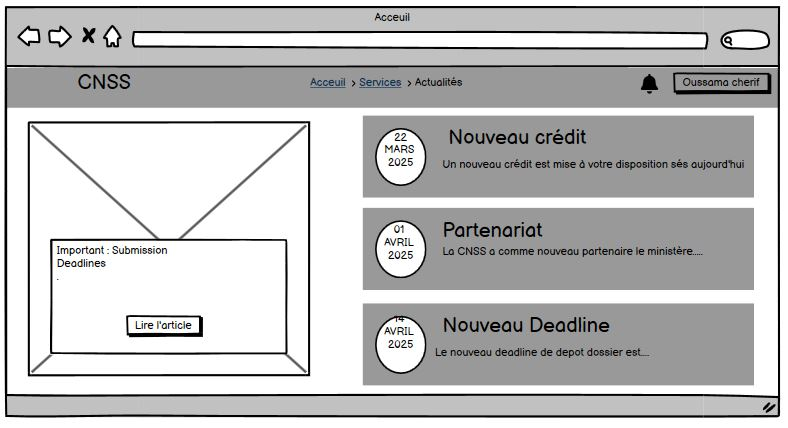
\includegraphics[width=0.9\textwidth]{figures/acceuil.JPG} 
    \caption{Prototype of consulting the Home Page.}
\end{figure}\
\begin{figure}[h]
    \centering
    \includegraphics[width=0.9\textwidth]{figures/actualité.JPG} 
    \caption{Prototype of consulting the Actuality Page.}
\end{figure}\
\clearpage
\begin{figure}[h]
    \centering
    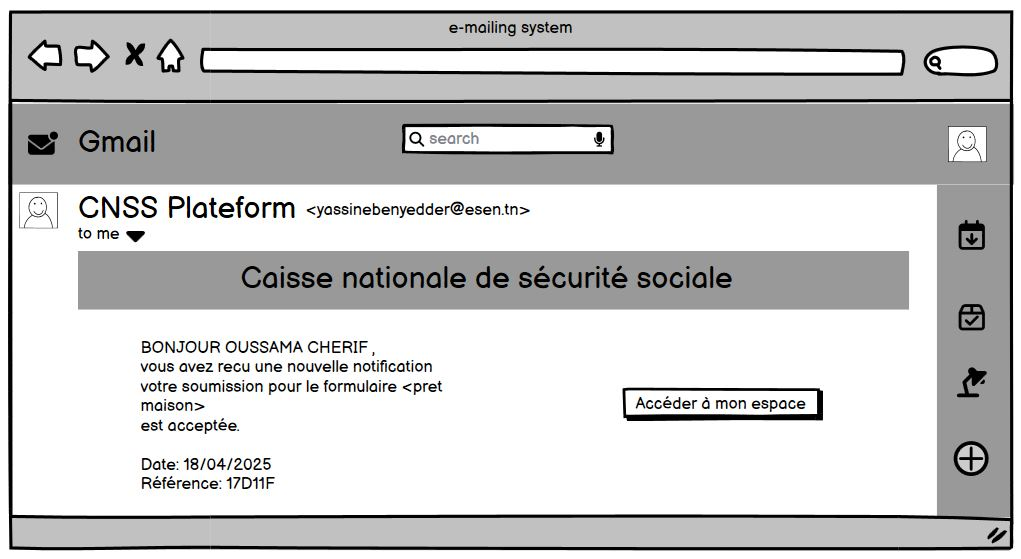
\includegraphics[width=0.9\textwidth]{figures/e-mailing system.JPG} 
    \caption{Prototype of the e-mailing system Page.}
\end{figure}\
\begin{figure}[h]
    \centering
    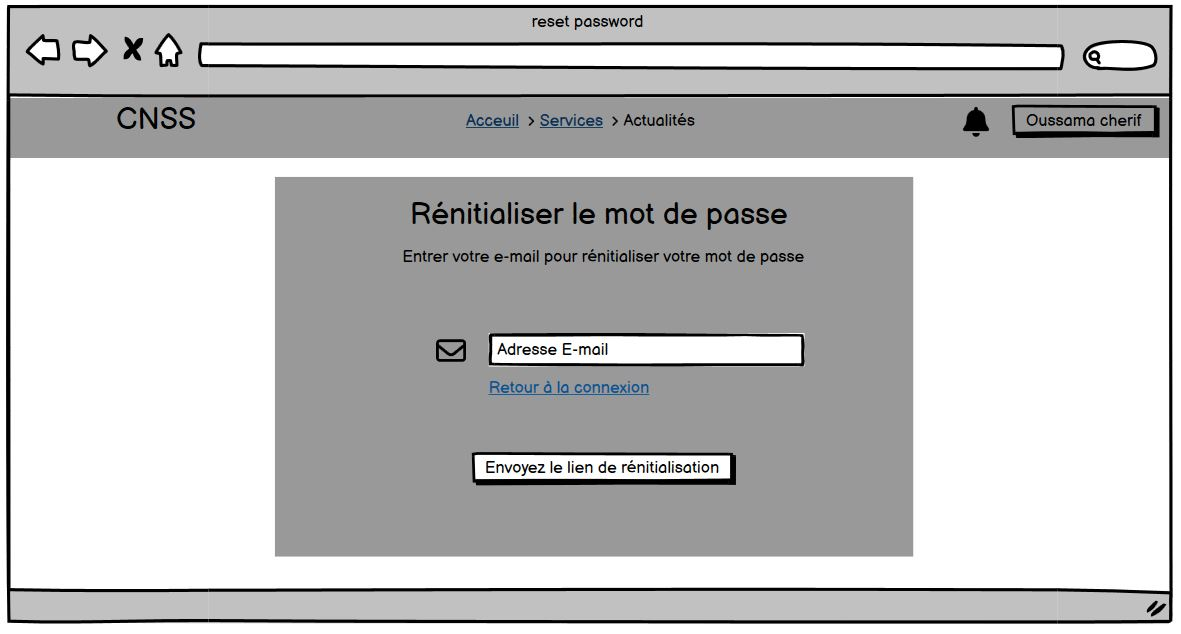
\includegraphics[width=0.9\textwidth]{figures/reset password.JPG} 
    \caption{Prototype of resetting the password Page.}
\end{figure}\
\clearpage
\begin{figure}[h]
    \centering
    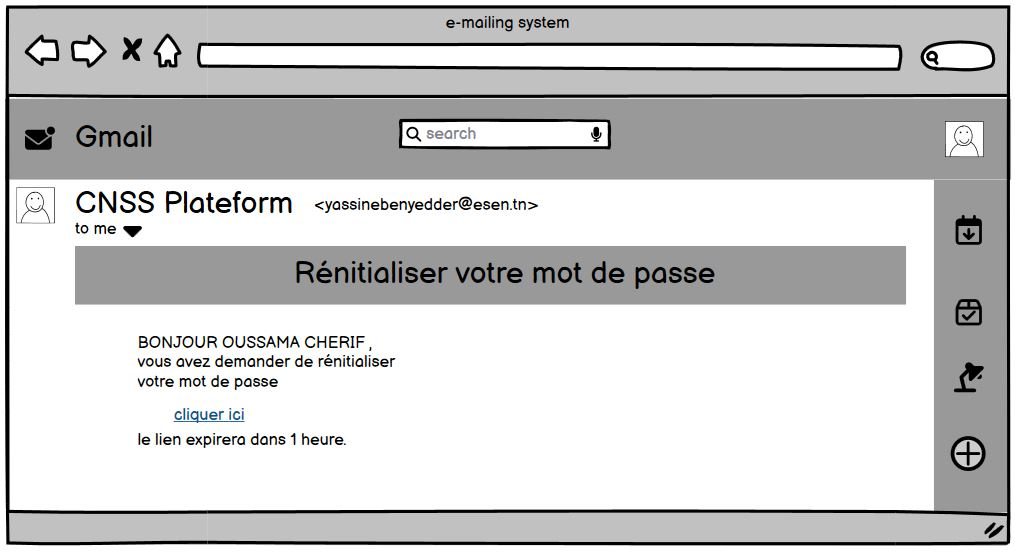
\includegraphics[width=0.9\textwidth]{figures/reset pass 2.JPG} 
    \caption{Prototype of resetting the password Page.}
\end{figure}\
\begin{figure}[h]
    \centering
    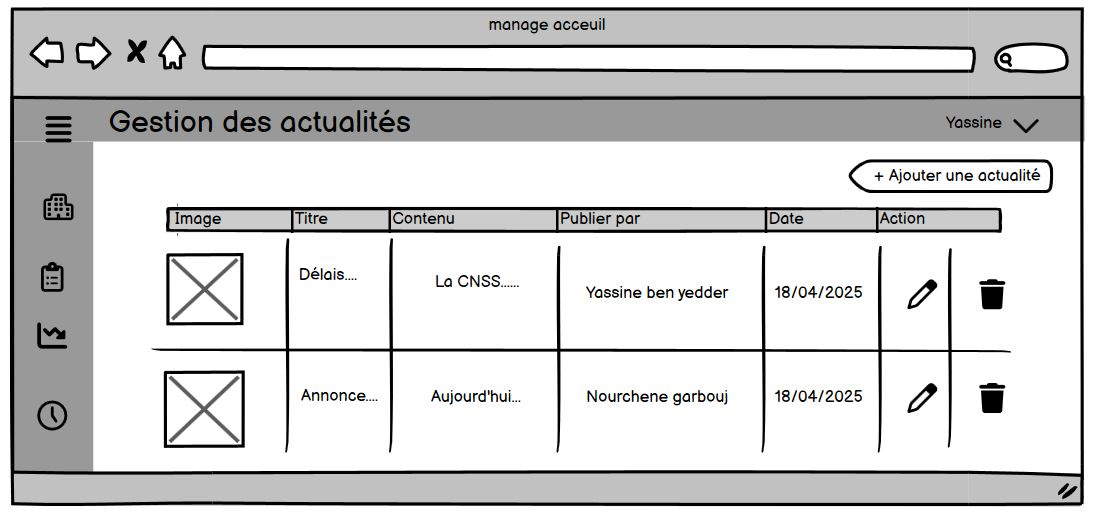
\includegraphics[width=0.9\textwidth]{figures/manage acceuil.JPG} 
    \caption{Prototype of managing the news Page.}
\end{figure}\
\clearpage
\begin{figure}[h]
    \centering
    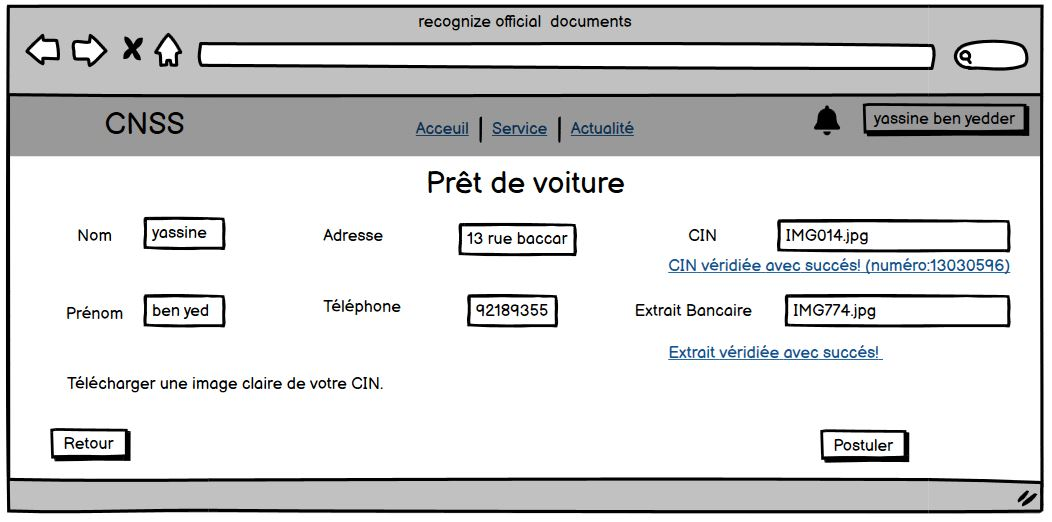
\includegraphics[width=0.9\textwidth]{figures/AI.JPG} 
    \caption{Prototype of recognizing national documents form.}
\end{figure}\

\section{Use Case Diagram of the Third Sprint}
This table provides a general classification of functionalities by actor.
 \begin{figure}[h]
    \centering
    \includegraphics[width=0.6\textwidth]{figures/table des cas d’utilisation du sprint 3.png}
    \caption{Classification of the use cases per actor.}
\end{figure}\
\clearpage
\begin{figure}[h!]
    \centering
    \includegraphics[width=0.9\textwidth]{figures/Diagramme des cas d’utilisation du sprint 3.png}
    \caption{Use Case Diagram of the Third Sprint}
\end{figure}\
\section{Use Case Analysis}
For each use case, we will provide a textual description in order to explain the scenario for each one and the exceptions that may arise.
\subsection{Use Case Analysis "Track submission status"}
\subsubsection{Textual Description of the "Consult News" Use Case}
\begin{table}[h]
\centering
\begin{tabular}{|l|p{8cm}|}
\hline
\textbf{Use Case} & See the news \\ \hline
\textbf{Actor} & Insured \\ \hline
\textbf{Pre-condition} & The insured user is authenticated. \\ \hline
\textbf{Post-condition} & The system displays the news list. \\ \hline
\textbf{Main Scenario Description} & 
\begin{tabular}[c]{@{}l@{}}
1. The insured opens the home page.\\
2. The system displays the news list.
\end{tabular} \\ \hline
\textbf{Alternative Scenarios} & None specified. \\ \hline
\end{tabular}
\caption{Use Case: See the news}
\end{table}
\clearpage
\begin{figure}[h]
    \centering
    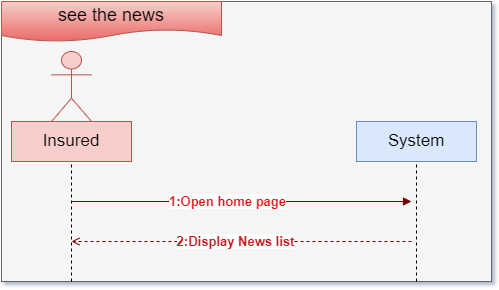
\includegraphics[width=0.9\textwidth]{figures/seq see the news.png}
    \caption{Sequence Diagram of the use case 'Consult News'}
\end{figure}\
\subsection{Use Case Analysis "Receive E-mails about my submission"}
\subsubsection{Textual Description of the "Receive E-mails about my submission" Use Case}
\begin{table}[h]
\centering
\begin{tabular}{|l|p{8cm}|}
\hline
\textbf{Use Case} & Receive emails about my submissions \\ \hline
\textbf{Actor} & Insured \\ \hline
\textbf{Pre-condition} & The submission has been accepted or refused. \\ \hline
\textbf{Post-condition} & An email is sent to the insured. \\ \hline
\textbf{Main Scenario Description} & 
\begin{tabular}[c]{@{}l@{}}
1. The system triggers the sending of an email.\\
2. The system sends the email via SMTP.\\
3. The email is sent successfully.
\end{tabular} \\ \hline
\textbf{Alternative Scenarios} & None specified. \\ \hline
\end{tabular}
\caption{Use Case: Receive emails about my submissions}
\end{table}
\clearpage
\begin{figure}[h]
    \centering
    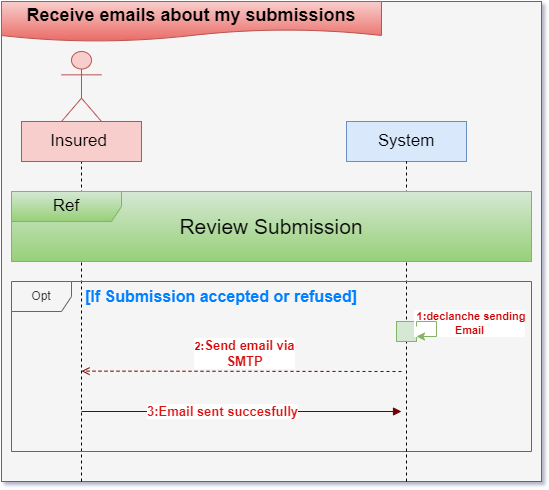
\includegraphics[width=0.9\textwidth]{figures/seq Receive emails about my submissions.png}
    \caption{Sequence Diagram of the use case 'Receive e-mails about my submissions'}
\end{figure}\
\clearpage
\subsection{Use Case Analysis: "Reset forgotten password"}
\subsubsection{Textual Description of the "Reset forgotten password" Use Case}
\begin{table}[h]
\centering
\begin{tabular}{|l|p{8cm}|}
\hline
\textbf{Use Case} & Reset forgotten password \\ \hline
\textbf{Actor} & Insured \\ \hline
\textbf{Pre-condition} & The insured has forgotten their password and has access to their registered email. \\ \hline
\textbf{Post-condition} & The insured's password is successfully updated. \\ \hline
\textbf{Main Scenario Description} & 
\begin{tabular}[c]{@{}l@{}}
1. Insured clicks "Forgot Password".\\
2. Insured enters email address.\\
3. System sends reset password link via email.\\
4. Insured clicks the link from the email.\\
5. System verifies the link.\\
6. Insured enters new password and confirms.\\
7. System displays "password updated \\successfully".
\end{tabular} \\ \hline
\textbf{Alternative Scenarios} & 
\begin{tabular}[c]{@{}l@{}}
6.a.1: Passwords do not match: System displays\\ "password doesn't match".\\
6.a.2: Password less than 8 characters: System \\displays "password must be 8 characters at \\least".\\
5.a.1: Link expired (clicked after 1 hour): \\System displays "link expired".\\
5.a.2: Password updated successfully even after\\ 1 hour: System displays "password updated \\successfully".
\end{tabular} \\ \hline
\end{tabular}
\caption{Use Case: Reset forgotten password}
\end{table}
\begin{figure}[h]
    \centering
    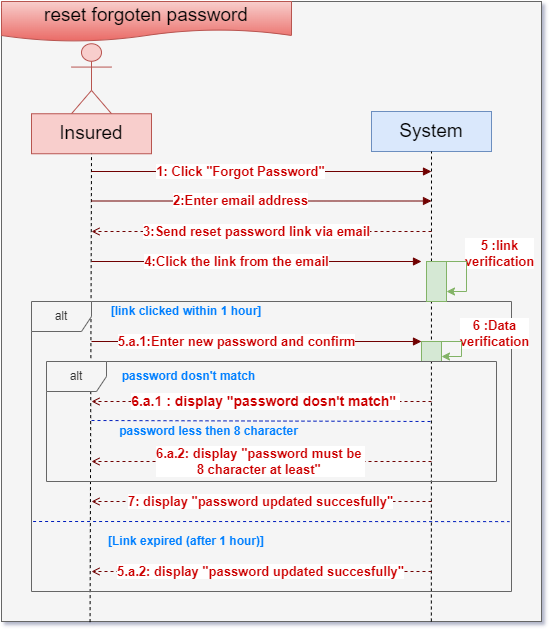
\includegraphics[width=1\textwidth]{figures/seq reset my forgoten password.png}
    \caption{Sequence Diagram of the use case 'Reset forgotten password'}
\end{figure}\
\clearpage

\subsection{Use Case Analysis: "Manage News on the platform"}
\subsubsection{Refinement of the use case 'Manage News on the platform'}
\begin{figure}[h]
    \centering
    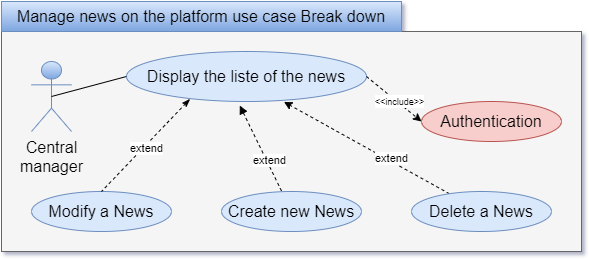
\includegraphics[width=1\textwidth]{figures/seq manages News-break down.png}
    \caption{Refinement of the use case 'Manage News on the platform'}
\end{figure}\
\subsubsection{Textual Description of the "Create News" Use Case}
\begin{table}[h]
\centering
\begin{tabular}{|l|p{8cm}|}
\hline
\textbf{Use Case} & Create a news \\ \hline
\textbf{Actor} & Central Manager \\ \hline
\textbf{Pre-condition} & The central manager is logged into the system. \\ \hline
\textbf{Post-condition} & The new news is displayed in the news list. \\ \hline
\textbf{Main Scenario Description} & 
\begin{tabular}[c]{@{}l@{}}
1. The central manager clicks "create new news"\\ button.\\
2. The system displays a form to create new \\news.\\
3. The central manager fills the form.\\
4. The central manager clicks confirm button.\\
5. The system verifies the data.\\
6. The system displays "Form created" and \\shows the new news.
\end{tabular} \\ \hline
\textbf{Alternative Scenarios} & 
\begin{tabular}[c]{@{}l@{}}
4.a.1. The central manager clicks cancel, the \\system redirects to the news list page.\\
5.a.1. Missing data: The system displays \\"Please fill in this field".
\end{tabular} \\ \hline
\end{tabular}
\caption{Use Case: Create a news}
\end{table}
\begin{figure}[h]
    \centering
    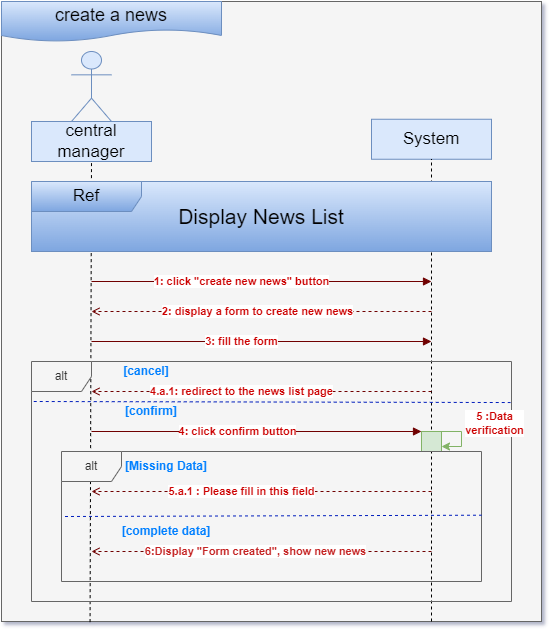
\includegraphics[width=1\textwidth]{figures/seq create a news.png}
    \caption{Sequence Diagram of the use case 'Create News'}
\end{figure}\
\clearpage

\subsubsection{Textual Description of the "Update News" Use Case}
\begin{table}[h]
\centering
\begin{tabular}{|l|p{8cm}|}
\hline
\textbf{Use Case} & Update a news \\ \hline
\textbf{Actor} & Central Manager \\ \hline
\textbf{Pre-condition} & The central manager is logged into the system and the news list is displayed. \\ \hline
\textbf{Post-condition} & The selected news is updated in the news list. \\ \hline
\textbf{Main Scenario Description} & 
\begin{tabular}[c]{@{}l@{}}
1. The central manager clicks "update news"\\ button.\\
2. The system displays a form to update the\\ news.\\
3. The central manager fills the form.\\
4. The central manager clicks confirm button.\\
5. The system verifies the data.\\
6. The system displays "news updated".
\end{tabular} \\ \hline
\textbf{Alternative Scenarios} & 
\begin{tabular}[c]{@{}l@{}}
4.a.1. The central manager clicks cancel, the\\ system redirects to the news list page.\\
5.a.1. Missing data: The system displays\\ "Please fill in this field".
\end{tabular} \\ \hline
\end{tabular}
\caption{Use Case: Update a news}
\end{table}
\begin{figure}[h]
    \centering
    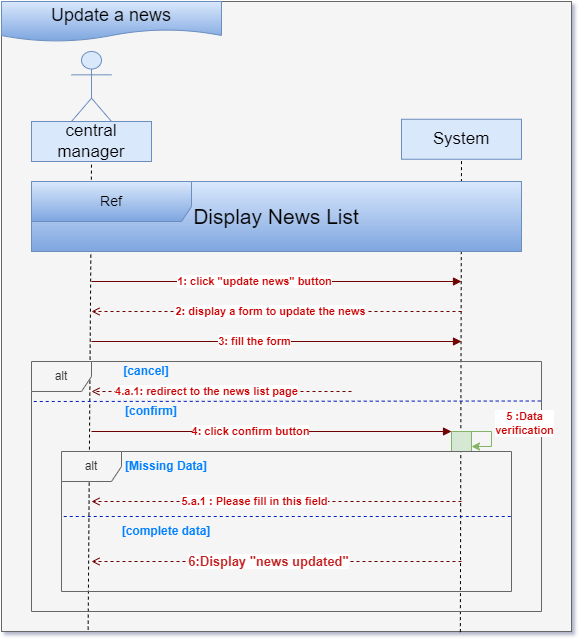
\includegraphics[width=1\textwidth]{figures/seq update a news.png}
    \caption{Sequence Diagram of the use case 'Update News'}
\end{figure}\
\clearpage

\subsubsection{Textual Description of the "Delete News" Use Case}
\begin{table}[h]
\centering
\begin{tabular}{|l|p{8cm}|}
\hline
\textbf{Use Case} & Delete a news \\ \hline
\textbf{Actor} & Central Manager \\ \hline
\textbf{Pre-condition} & The central manager is logged into the system and the news list is displayed. \\ \hline
\textbf{Post-condition} & The selected news is deleted from the news list. \\ \hline
\textbf{Main Scenario Description} & 
\begin{tabular}[c]{@{}l@{}}
1. The central manager clicks "Delete" on a\\ news item.\\
2. The system displays "Are you sure you want \\to delete this news?".\\
3. The central manager selects confirm.\\
4. The system displays "News deleted \\successfully".
\end{tabular} \\ \hline
\textbf{Alternative Scenarios} & 
\begin{tabular}[c]{@{}l@{}}
3.a.1. The central manager selects cancel, \\the system redirects to the news list page.
\end{tabular} \\ \hline
\end{tabular}
\caption{Use Case: Delete a news}
\end{table}
\begin{figure}[h]
    \centering
    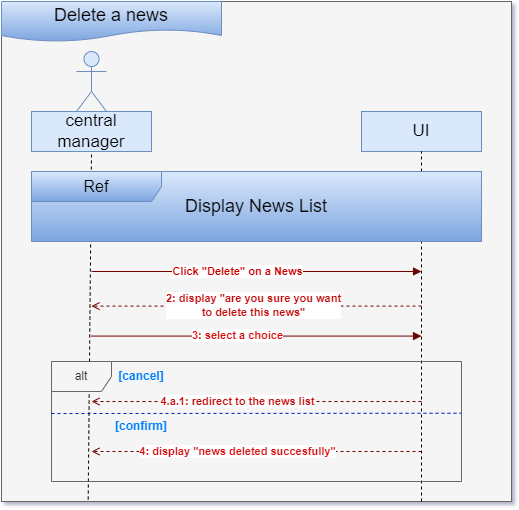
\includegraphics[width=1\textwidth]{figures/seq delete a news.png}
    \caption{Sequence Diagram of the use case 'Delete News'}
\end{figure}\
\clearpage

\subsection{Use Case Analysis "Recognize national identity documents"}
\subsubsection{Textual Description of the "Recognize national identity documents" Use Case}
\begin{table}[h]
\centering
\begin{tabular}{|l|p{8cm}|}
\hline
\textbf{Use Case} & Validate national identity documents \\ \hline
\textbf{Actor} & System \\ \hline
\textbf{Pre-condition} & National identity documents have been uploaded to the system. \\ \hline
\textbf{Post-condition} & Documents are validated and important data is extracted. \\ \hline
\textbf{Main Scenario Description} & 
\begin{tabular}[c]{@{}l@{}}
1. The system sends uploaded documents to\\ OpenAI API.\\
2. OpenAI API processes the documents.\\
3. OpenAI API returns validation status \\(valid/invalid) and extracted data.\\
4. The system receives and processes the API \\response.
\end{tabular} \\ \hline
\textbf{Alternative Scenarios} & 
\begin{tabular}[c]{@{}l@{}}
2.a.1. If documents are unreadable, API returns\\ error status.
\end{tabular} \\ \hline
\end{tabular}
\caption{Use Case: Validate national identity documents}
\end{table}
\begin{figure}[h]
    \centering
    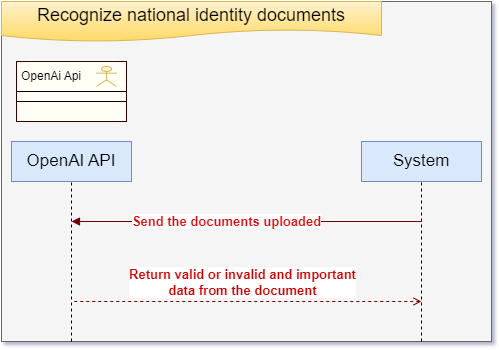
\includegraphics[width=0.7\textwidth]{figures/seq validate national identity documents.png}
    \caption{Sequence Diagram of the use case 'Recognize national identity documents'}
\end{figure}\
\clearpage

\section{Design of Use Cases}
\subsection{The participant Class Diagram}
\subsubsection{Participant class Diagram for the use case "Consult News"}
\begin{figure}[h!]
    \centering
    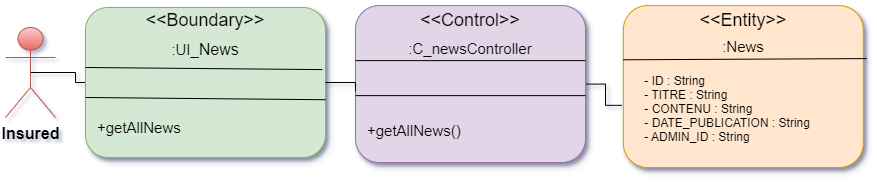
\includegraphics[width=1\textwidth]{figures/dc see the news.png}
    \caption{Participant class Diagram for the use case "Consult News"}
\end{figure}\
\subsubsection{Participant class Diagram for the use case "Receive e-mails about my submissions"}
\begin{figure}[h!]
    \centering
    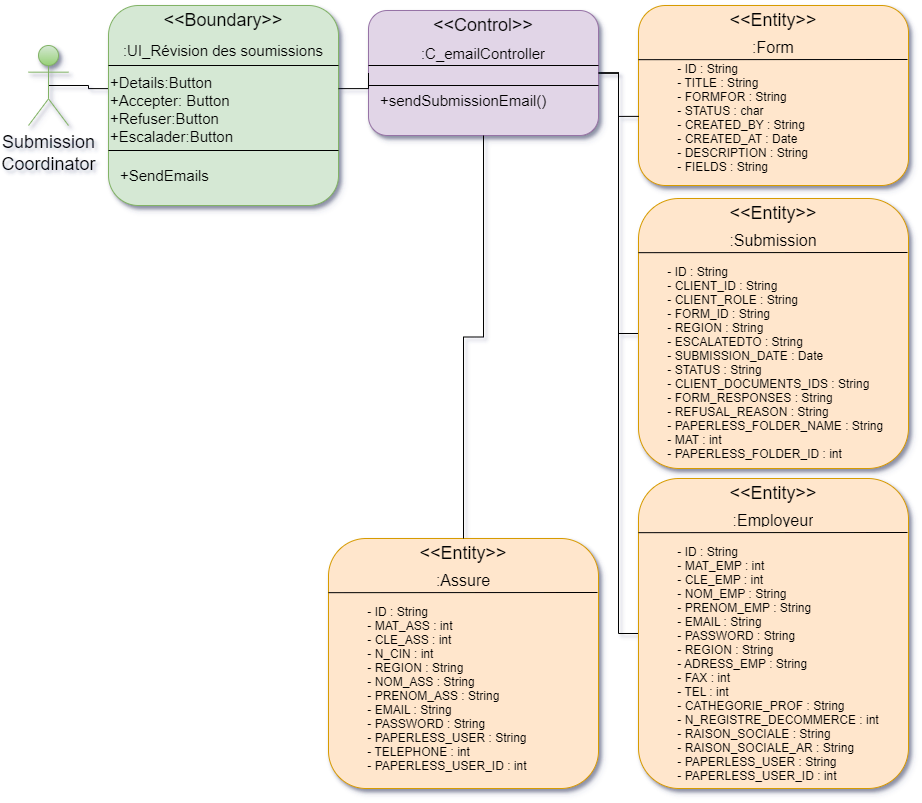
\includegraphics[width=0.9\textwidth]{figures/dc Receive emails about my submissions.png}
    \caption{Participant class Diagram for the use case "Receive e-mails about my submissions"}
    \clearpage
\end{figure}\
\subsubsection{Participant class Diagram for the use case "Reset forgotten password"}
\begin{figure}[h!]
    \centering
    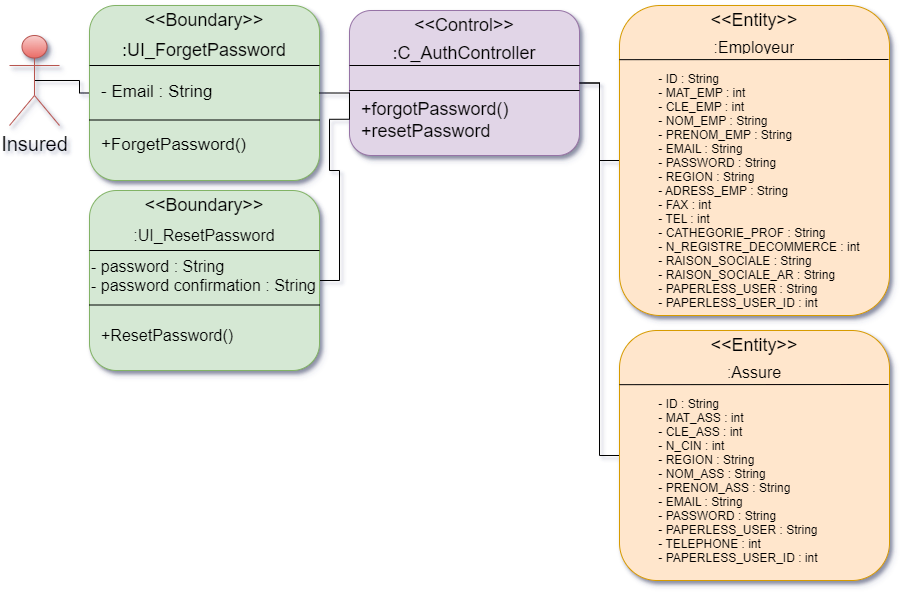
\includegraphics[width=1\textwidth]{figures/dc reset my forgoten password.png}
    \caption{Participant class Diagram for the use case "Reset forgotten password"}
\end{figure}\
\subsubsection{Participant class Diagram for the use case "Manage news on the platform"}
\begin{figure}[h]
    \centering
    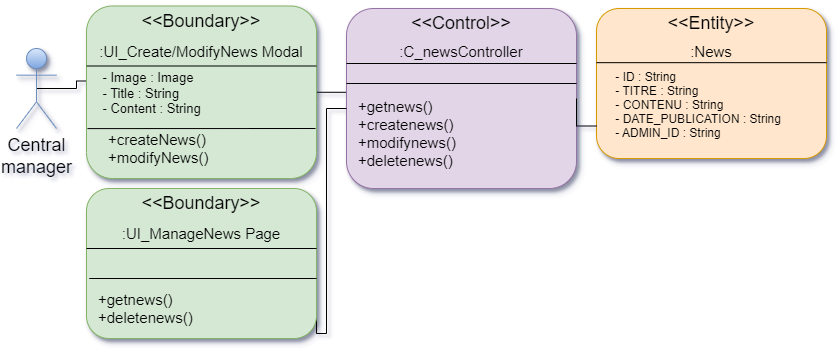
\includegraphics[width=1\textwidth]{figures/dc manages News.png}
    \caption{Participant class Diagram for the use case "Manage news on the platform"}
\end{figure}\
\subsubsection{Participant class Diagram for the use case "Recognize national identity documents"}
\begin{figure}[h]
    \centering
    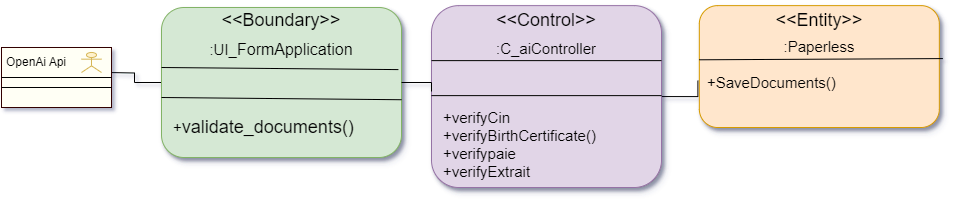
\includegraphics[width=1\textwidth]{figures/dc validate national identity documents.png}
    \caption{Participant class Diagram for the use case "Recognize national identity documents"}
\end{figure}\

\subsection{Detailed Sequence Diagram}
\subsubsection{Detailed sequence diagram of the 'Consult News' use case}
\begin{figure}[h!]
    \centering
    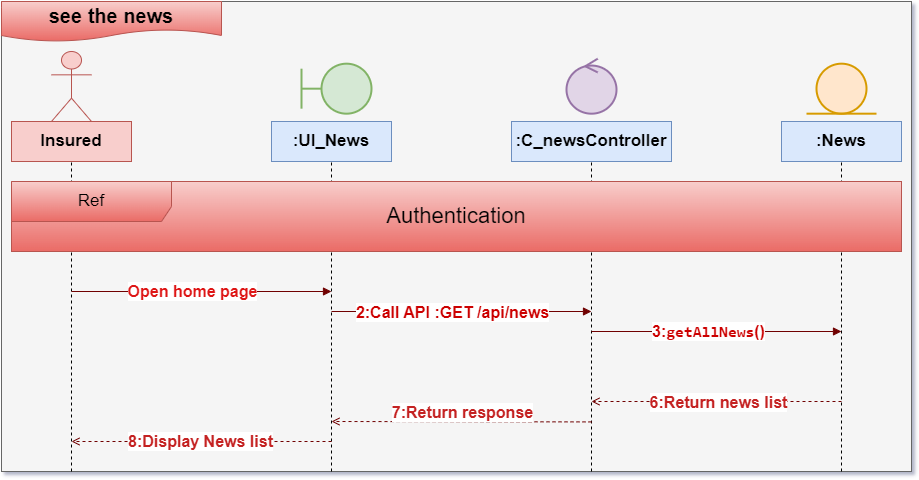
\includegraphics[width=1\textwidth]{figures/det see the news.png}
    \caption{Detailed sequence diagram of the 'Consult News' use case}
\end{figure}
\clearpage
\subsubsection{Detailed sequence diagram of the 'Receive e-mails about my submissions' use case}
\begin{figure}[h!]
    \centering
    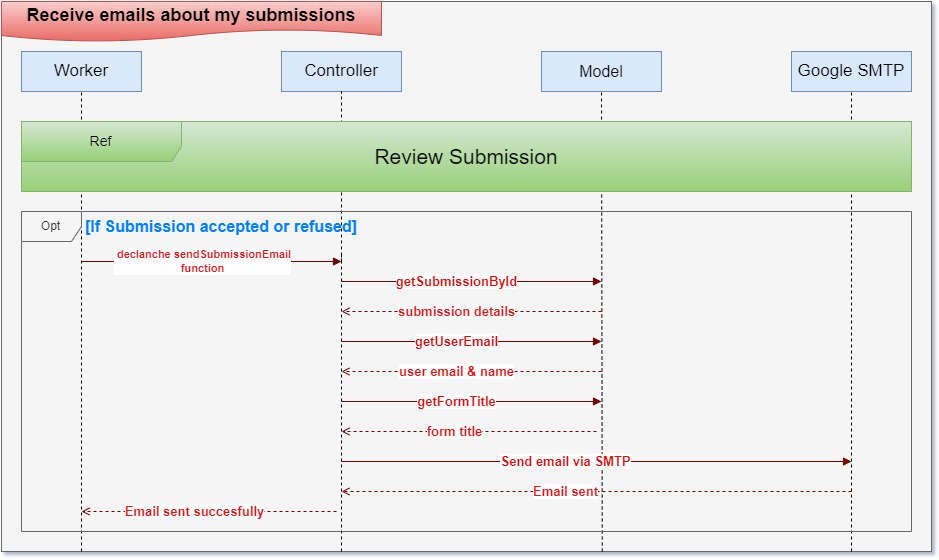
\includegraphics[width=1\textwidth]{figures/det Receive emails about my submissions.png}
    \caption{Detailed sequence diagram of the 'Receive e-mails about my submissions' use case}
\end{figure}
\subsubsection{Detailed sequence diagram of the 'Reset forgotten password' use case}
\begin{figure}[h!]
    \centering
    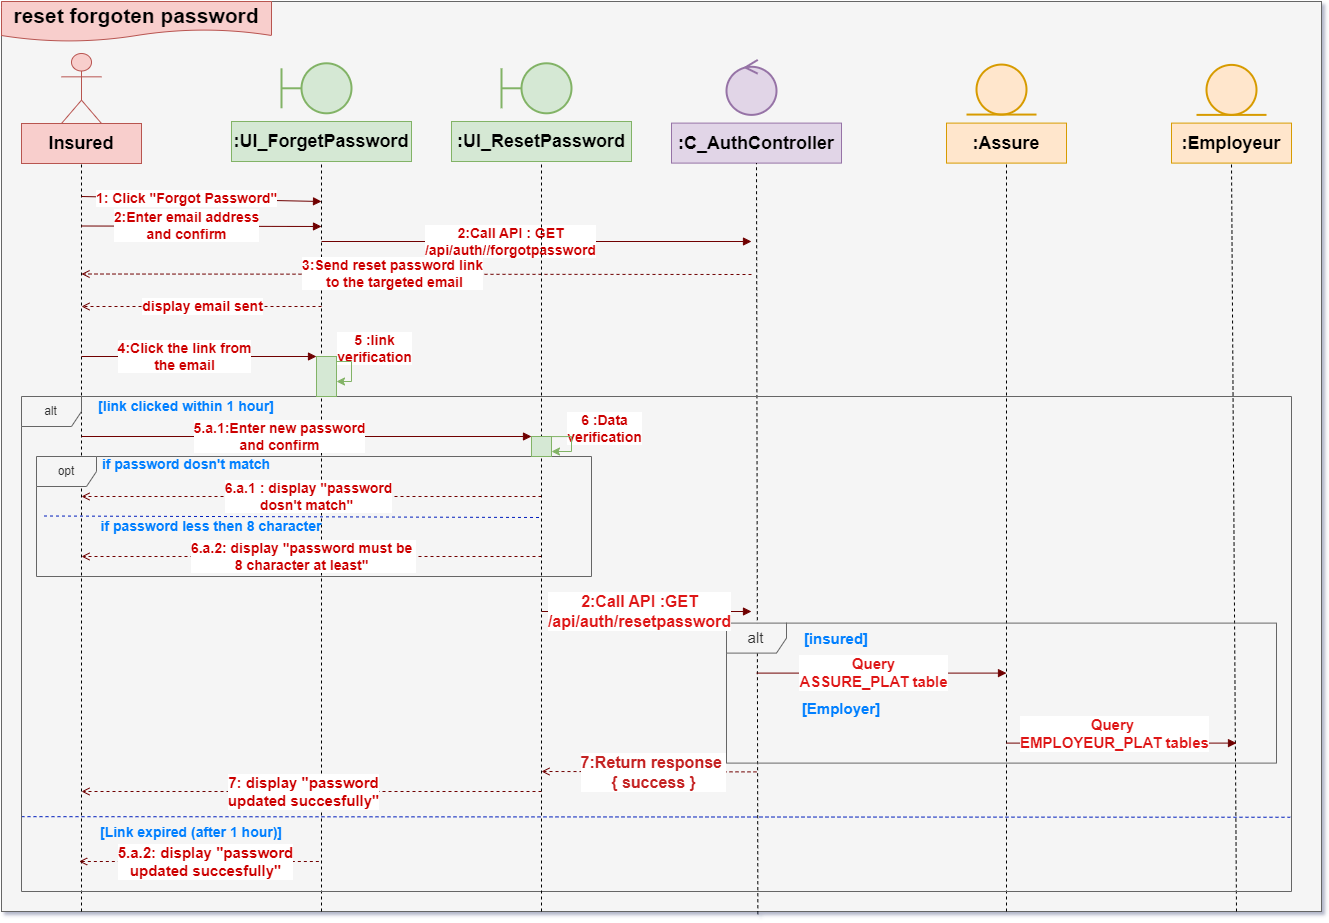
\includegraphics[width=0.8\textwidth]{figures/det reset my forgoten password.png}
    \caption{Detailed sequence diagram of the 'Reset forgotten password' use case}
\end{figure}
\clearpage
\subsubsection{Detailed sequence diagram of the 'Manage news on the platform' use case}
\begin{figure}[h!]
    \centering
    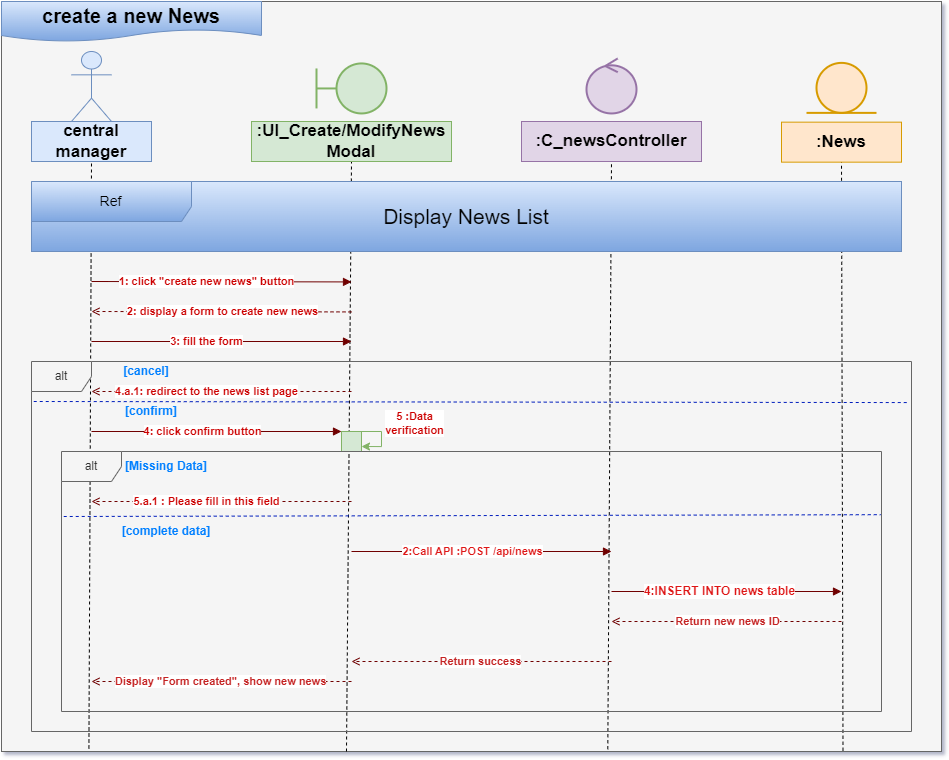
\includegraphics[width=0.8\textwidth]{figures/det create a news.png}
    \caption{Detailed sequence diagram of the 'Create news' use case}
\end{figure}
\begin{figure}[h!]
    \centering
    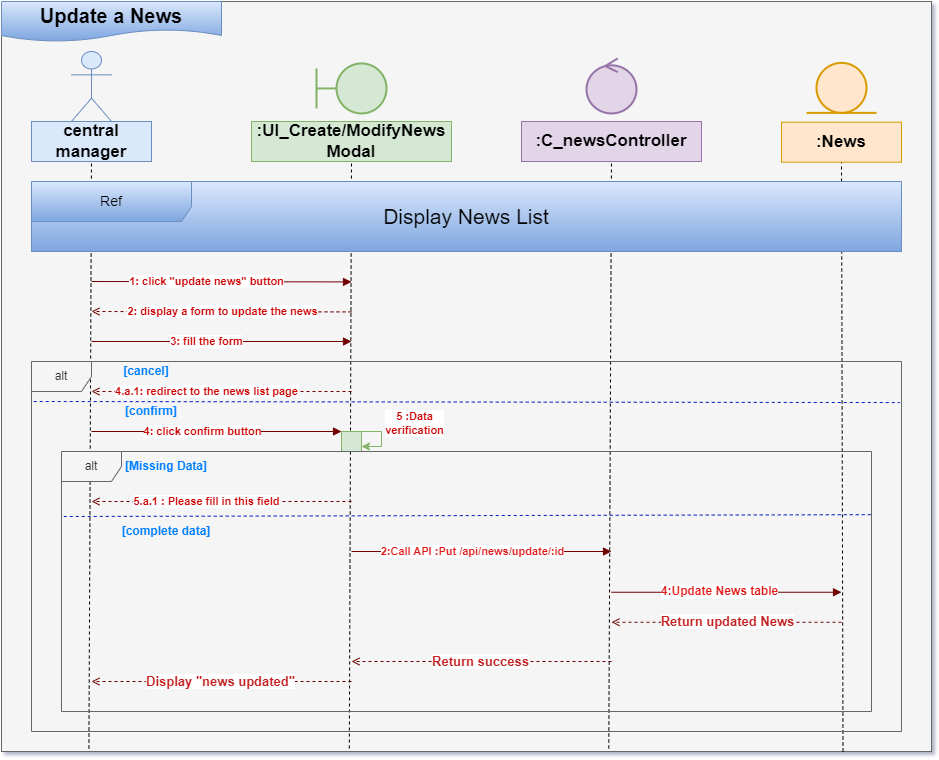
\includegraphics[width=0.8\textwidth]{figures/det update a news.png}
    \caption{Detailed sequence diagram of the 'Update news' use case}
\end{figure}
\clearpage
\begin{figure}[h!]
    \centering
    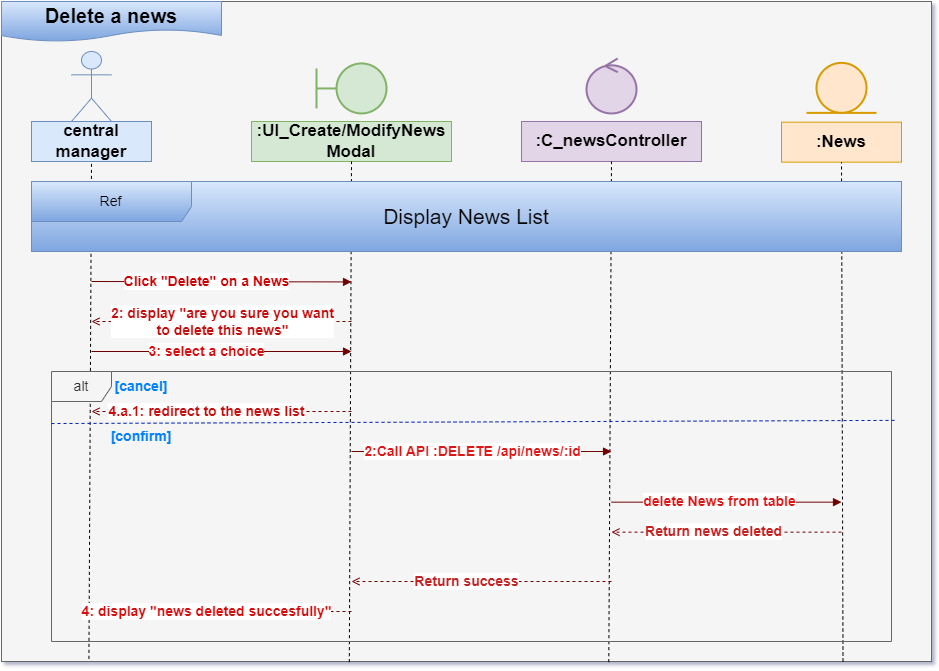
\includegraphics[width=1\textwidth]{figures/det delete a news.png}
    \caption{Detailed sequence diagram of the 'Delete news' use case}
\end{figure}
\clearpage
\section{Global class diagram of the third sprint}
\begin{figure}[h!]
    \centering
    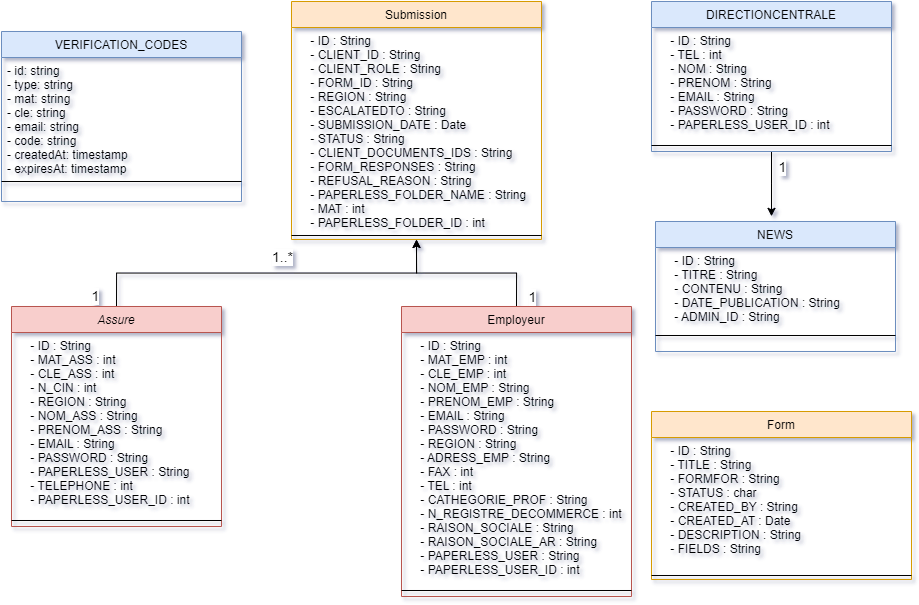
\includegraphics[width=1\textwidth]{figures/global class diagram sprint 3.png}
    \caption{Global class diagram of Sprint 3.}
\end{figure}


\section{Implementation}
In this step, we will define the structure of the current sprint's database while applying the rules for transforming the entity/association model into the relational model.
\subsection{The Database Schemas}
\begin{table}[h!]
\centering
\begin{tabular}{|l|l|l|}
\hline
\textbf{Attribut} & \textbf{Type} & \textbf{Contrainte} \\
\hline
id & VARCHAR & PRIMARY KEY \\
type & VARCHAR(50) & - \\
mat & VARCHAR(50) & - \\
cle & VARCHAR(50) & - \\
email & VARCHAR(100) & - \\
code & VARCHAR(50) & - \\
createdAt & TIMESTAMP & - \\
expiresAt & TIMESTAMP & - \\
\hline
\end{tabular}
\caption{Table \texttt{VERIFICATION\_CODES}}
\end{table}
\clearpage
\begin{table}[h!]
\centering
\begin{tabular}{|l|l|l|}
\hline
\textbf{Attribut} & \textbf{Type} & \textbf{Contrainte} \\
\hline
ID & VARCHAR & PRIMARY KEY \\
CLIENT\_ID & VARCHAR & FOREIGN KEY \\
CLIENT\_ROLE & VARCHAR(50) & - \\
FORM\_ID & VARCHAR & FOREIGN KEY \\
REGION & VARCHAR(50) & - \\
ESCALATEDTO & VARCHAR & - \\
SUBMISSION\_DATE & DATE & - \\
STATUS & VARCHAR(50) & - \\
CLIENT\_DOCUMENTS\_IDS & VARCHAR & - \\
FORM\_RESPONSES & TEXT & - \\
REFUSAL\_REASON & TEXT & - \\
PAPERLESS\_FOLDER\_NAME & VARCHAR(100) & - \\
MAT & INT & - \\
PAPERLESS\_FOLDER\_ID & INT & - \\
\hline
\end{tabular}
\caption{Table \texttt{Submission}}
\end{table}

\begin{table}[h!]
\centering
\begin{tabular}{|l|l|l|}
\hline
\textbf{Attribut} & \textbf{Type} & \textbf{Contrainte} \\
\hline
ID & VARCHAR & PRIMARY KEY \\
TEL & INT & - \\
NOM & VARCHAR(50) & Not Null \\
PRENOM & VARCHAR(50) & Not Null \\
EMAIL & VARCHAR(100) & UNIQUE - Not Null \\
PASSWORD & VARCHAR(255) & Not Null \\
PAPERLESS\_USER\_ID & INT & - \\
\hline
\end{tabular}
\caption{Table \texttt{DIRECTIONCENTRALE}}
\end{table}

\begin{table}[h!]
\centering
\begin{tabular}{|l|l|l|}
\hline
\textbf{Attribut} & \textbf{Type} & \textbf{Contrainte} \\
\hline
ID & VARCHAR & PRIMARY KEY \\
MAT\_ASS & INT & - \\
CLE\_ASS & INT & - \\
N\_CIN & INT & - \\
REGION & VARCHAR(50) & - \\
NOM\_ASS & VARCHAR(50) & Not Null \\
PRENOM\_ASS & VARCHAR(50) & Not Null \\
EMAIL & VARCHAR(100) & UNIQUE - Not Null \\
PASSWORD & VARCHAR(255) & Not Null \\
PAPERLESS\_USER & VARCHAR(100) & - \\
TELEPHONE & INT & - \\
PAPERLESS\_USER\_ID & INT & - \\
\hline
\end{tabular}
\caption{Table \texttt{Assure}}
\end{table}

\begin{table}[h!]
\centering
\begin{tabular}{|l|l|l|}
\hline
\textbf{Attribut} & \textbf{Type} & \textbf{Contrainte} \\
\hline
ID & VARCHAR & PRIMARY KEY \\
MAT\_EMP & INT & - \\
CLE\_EMP & INT & - \\
NOM\_EMP & VARCHAR(50) & Not Null \\
PRENOM\_EMP & VARCHAR(50) & Not Null \\
EMAIL & VARCHAR(100) & UNIQUE - Not Null \\
PASSWORD & VARCHAR(255) & Not Null \\
REGION & VARCHAR(50) & - \\
ADRESS\_EMP & TEXT & - \\
FAX & INT & - \\
TEL & INT & - \\
CATHEOORIE\_PROF & VARCHAR(50) & - \\
N\_REGISTRE\_DECOMMERCE & INT & - \\
RAISON\_SOCIALE & VARCHAR(100) & - \\
PAPERLESS\_USER & VARCHAR(100) & - \\
PAPERLESS\_USER\_ID & INT & - \\
\hline
\end{tabular}
\caption{Table \texttt{Employeur}}
\end{table}

\begin{table}[h!]
\centering
\begin{tabular}{|l|l|l|}
\hline
\textbf{Attribut} & \textbf{Type} & \textbf{Contrainte} \\
\hline
ID & VARCHAR & PRIMARY KEY \\
TITRE & VARCHAR(100) & Not Null \\
CONTENU & TEXT & Not Null \\
DATE\_PUBLICATION & VARCHAR(50) & - \\
ADMIN\_ID & VARCHAR & FOREIGN KEY \\
\hline
\end{tabular}
\caption{Table \texttt{NEWS}}
\end{table}
\clearpage
\begin{table}[h!]
\centering
\begin{tabular}{|l|l|l|}
\hline
\textbf{Attribut} & \textbf{Type} & \textbf{Contrainte} \\
\hline
ID & VARCHAR & PRIMARY KEY \\
TITLE & VARCHAR(100) & Not Null \\
FORMEOR & VARCHAR(50) & - \\
STATUS & CHAR(1) & - \\
CREATED\_BY & VARCHAR & FOREIGN KEY \\
CREATED\_AT & DATE & - \\
DESCRIPTION & TEXT & - \\
FIELDS & TEXT & - \\
\hline
\end{tabular}
\caption{Table \texttt{Form}}
\end{table}
\subsection{The interfaces of the use cases}
\begin{figure}[h!]
    \centering
    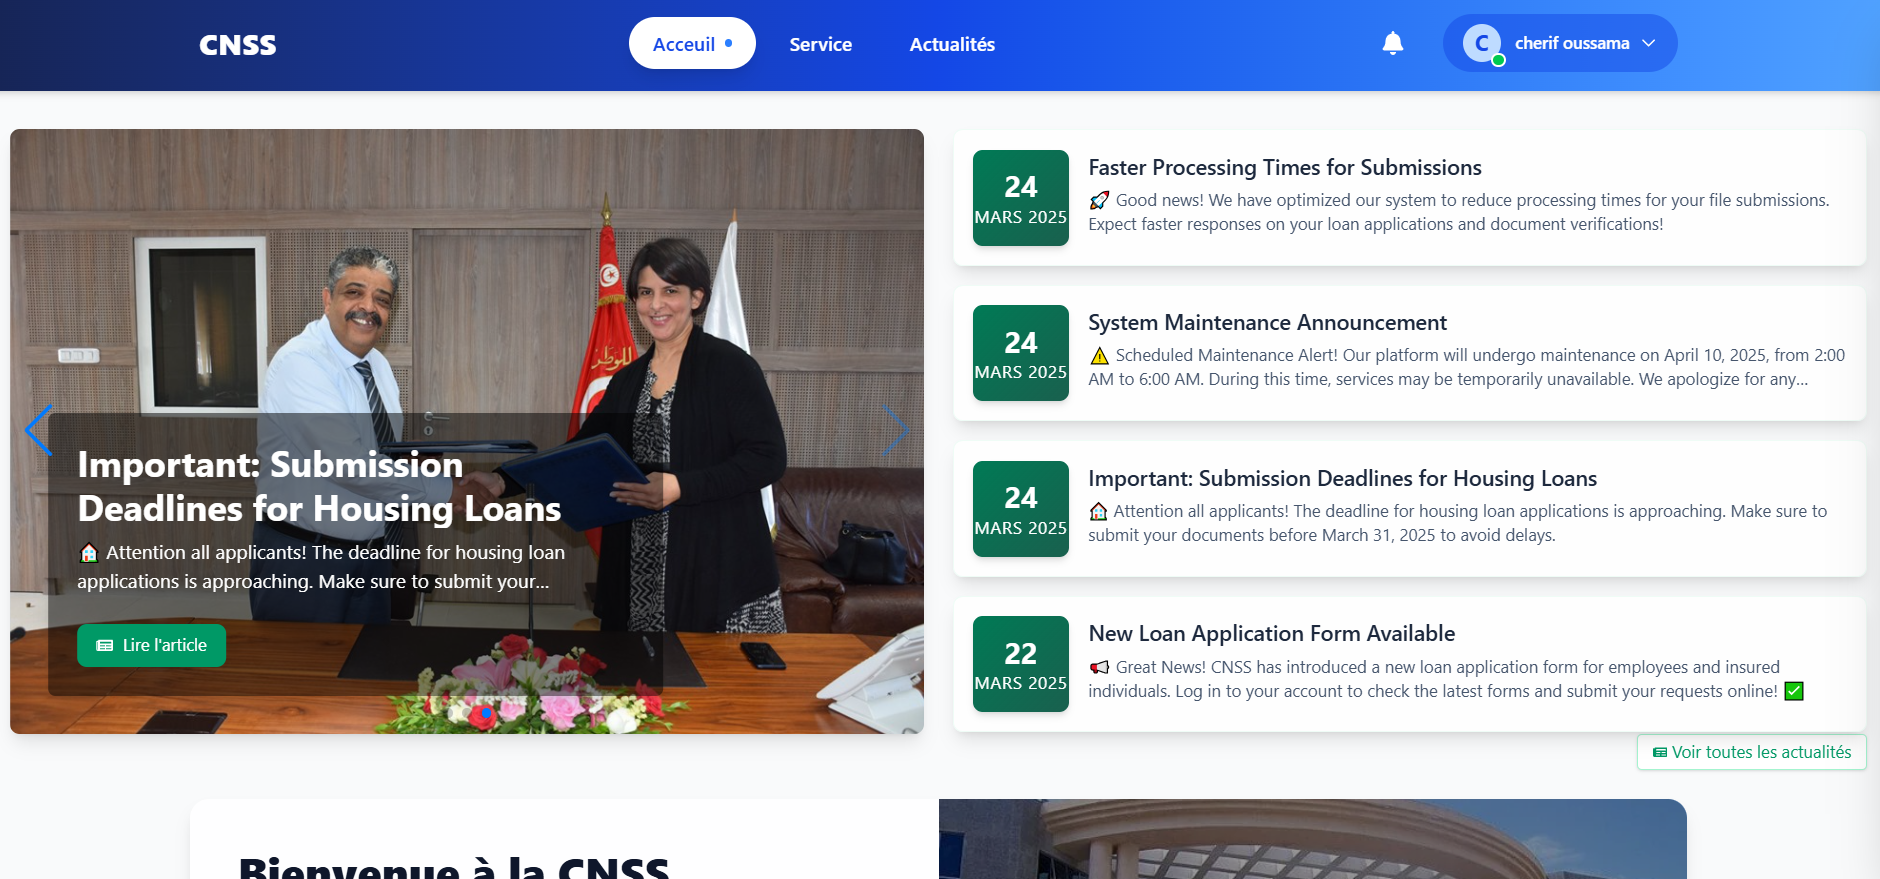
\includegraphics[width=1\textwidth]{figures/ui-see news1.png}
    \caption{Interface of consulting news 1.}
\end{figure}
\clearpage
\begin{figure}[h!]
    \centering
    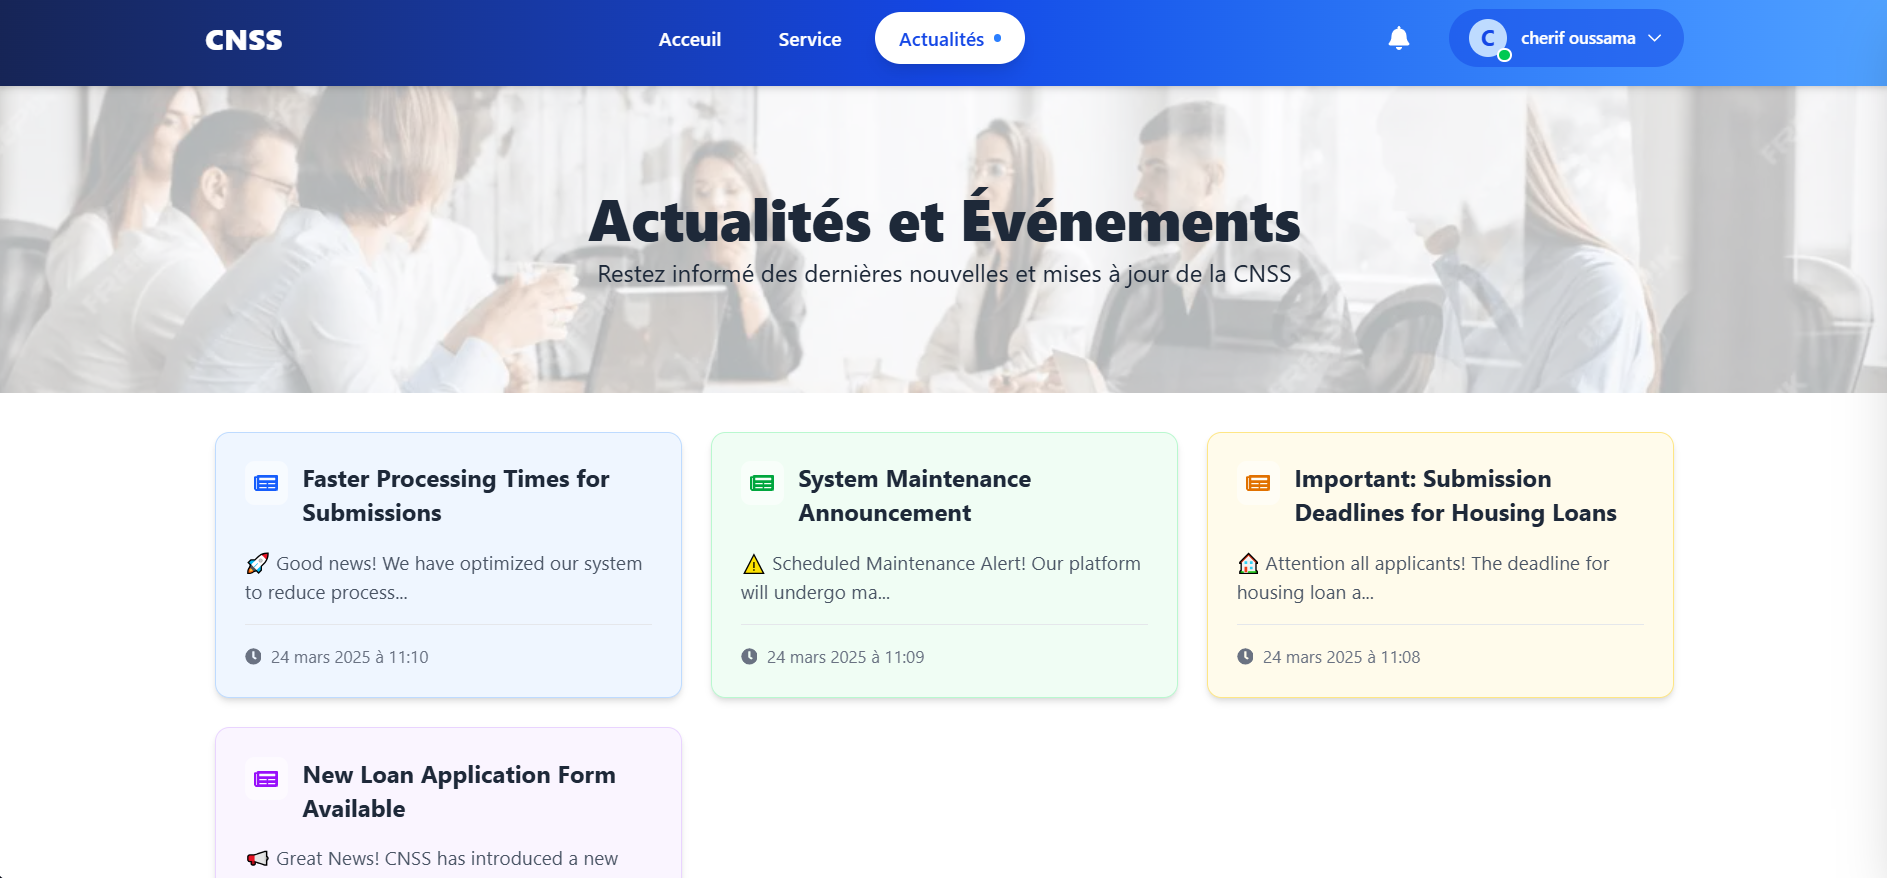
\includegraphics[width=1\textwidth]{figures/ui-see news2.png}
    \caption{Interface of consulting news 2.}
\end{figure}
\vspace{1.5cm}
\begin{figure}[h!]
    \centering
    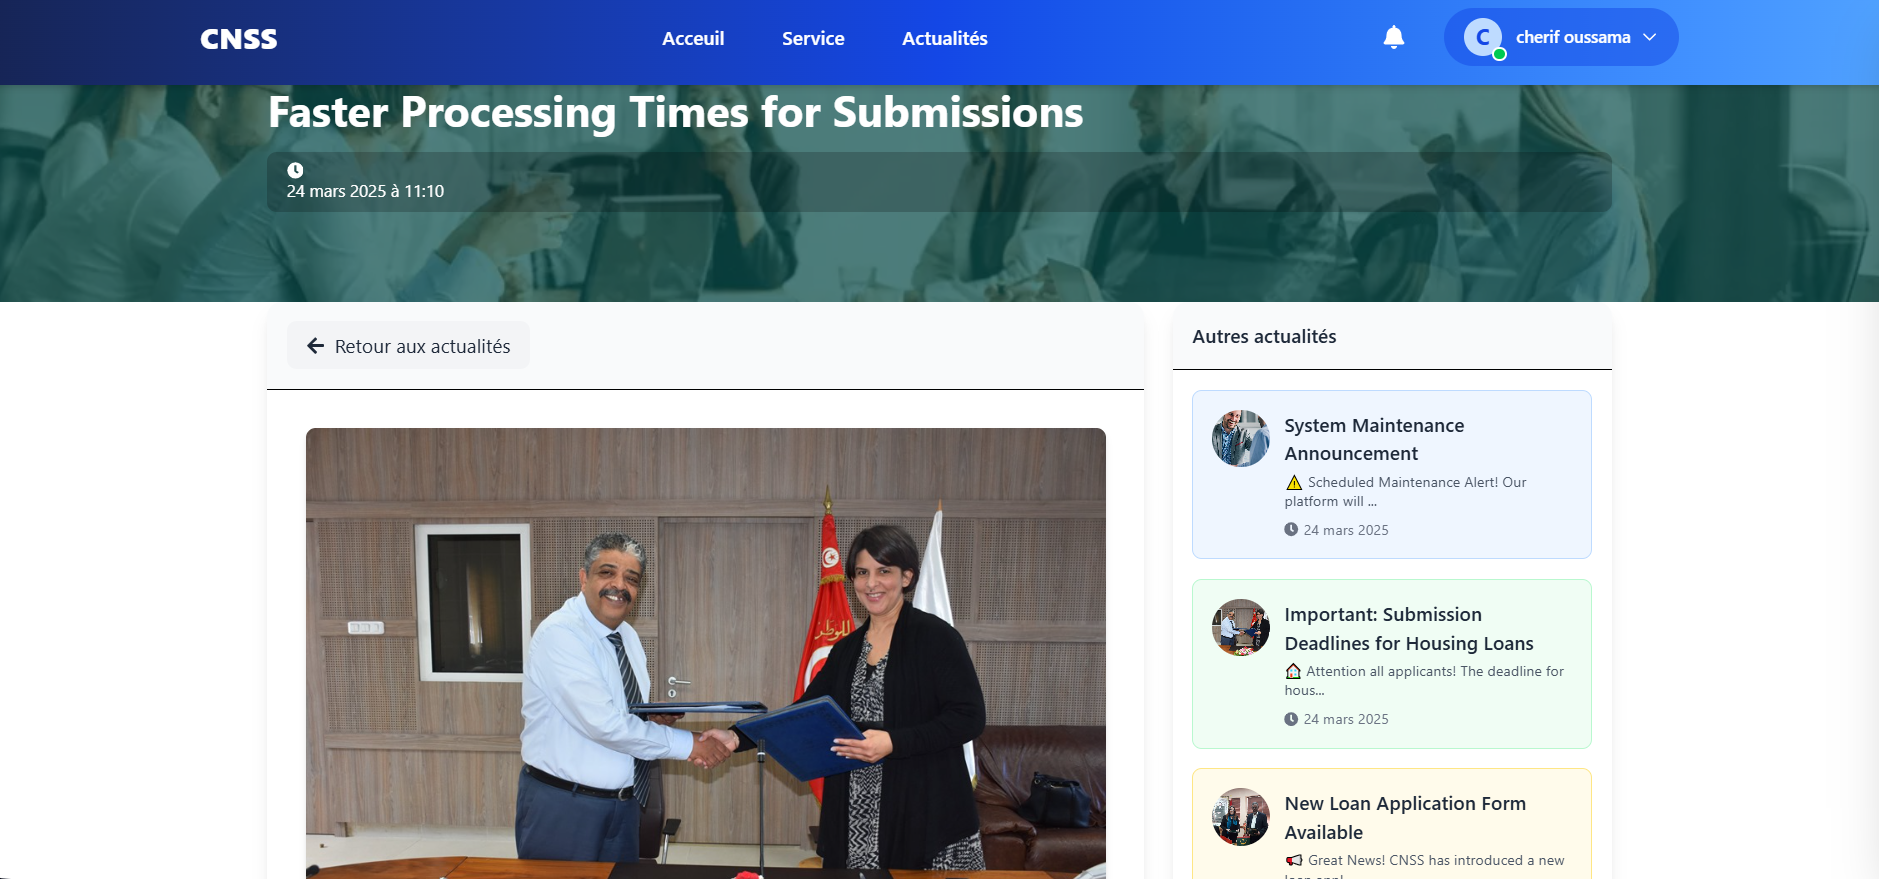
\includegraphics[width=1\textwidth]{figures/ui-see news3.png}
    \caption{Interface of consulting news 3.}
\end{figure}
\clearpage
\begin{figure}[h!]
    \centering
    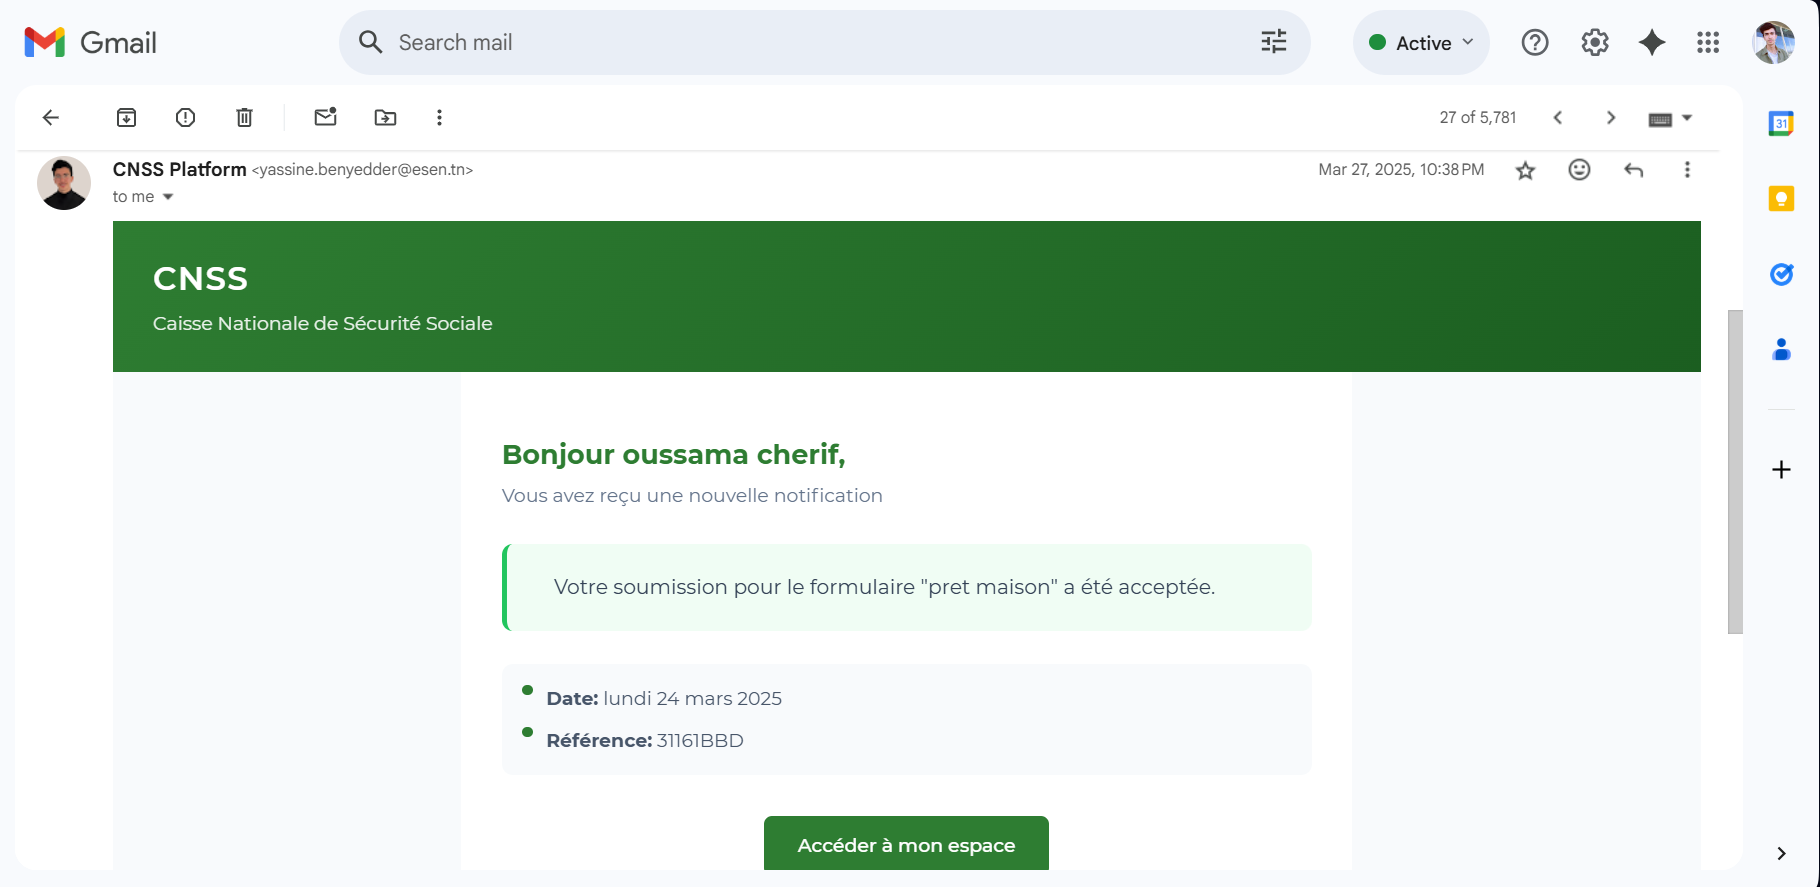
\includegraphics[width=1\textwidth]{figures/ui-receive emails.png}
    \caption{Interface of receiving an e-mail.}
\end{figure}
\vspace{1.5cm}
\begin{figure}[h!]
    \centering
    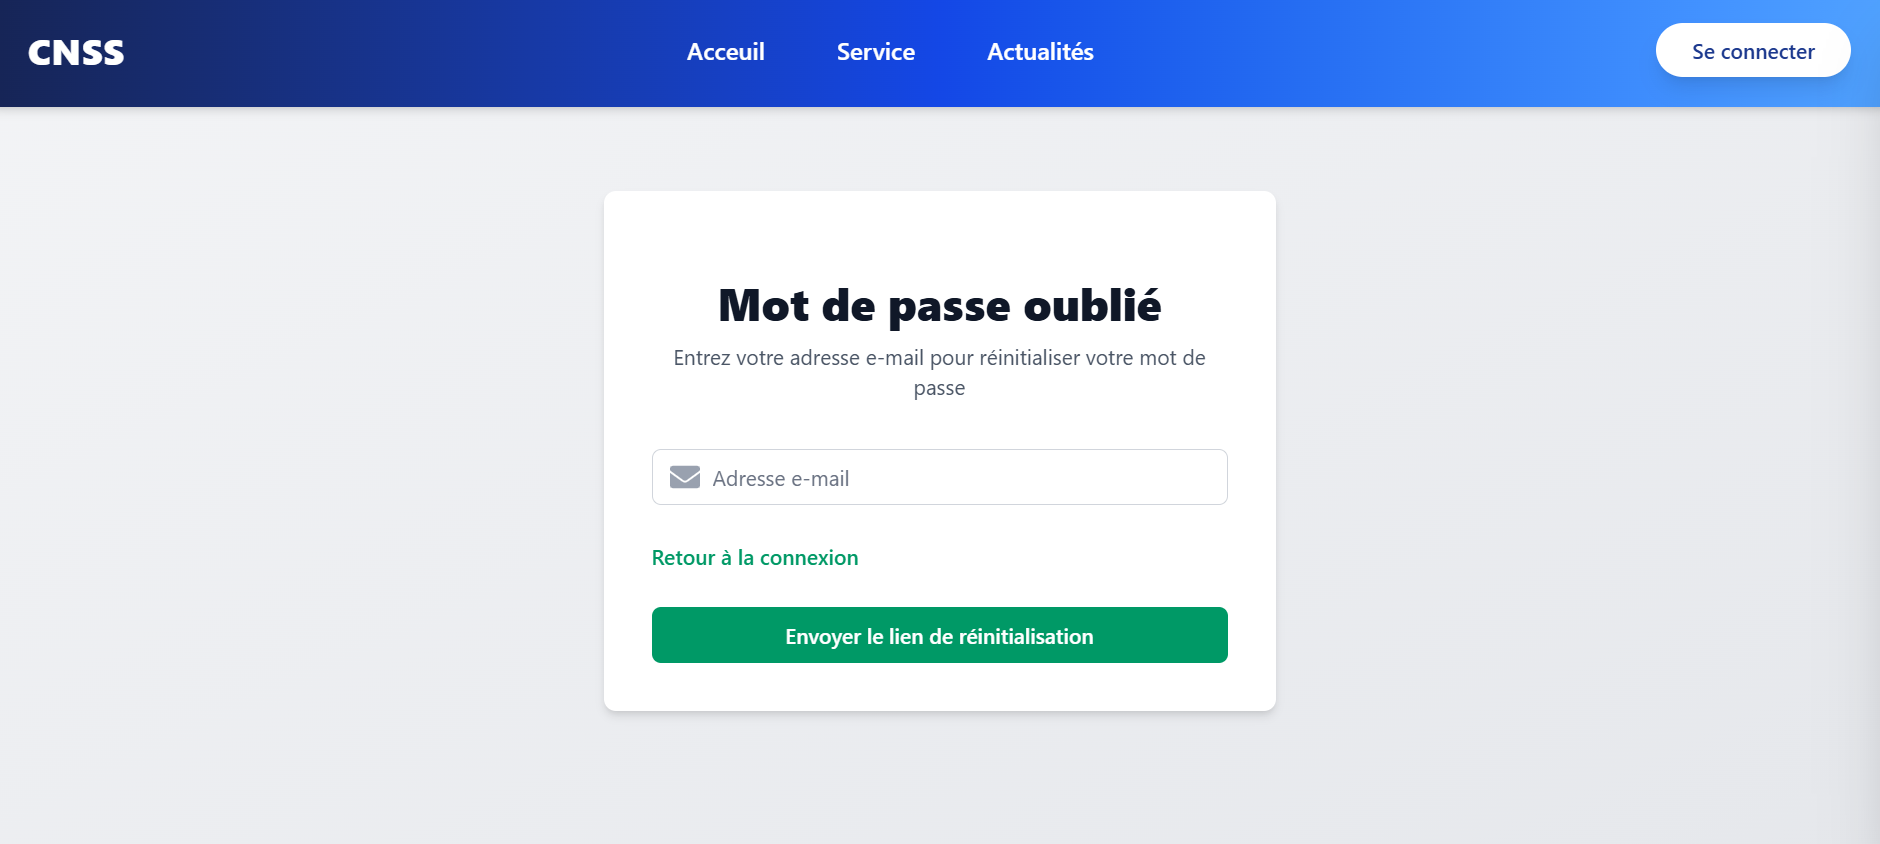
\includegraphics[width=1\textwidth]{figures/ui-reset pass1.png}
    \caption{Interface of resetting password 1.}
\end{figure}
\clearpage
\begin{figure}[h!]
    \centering
    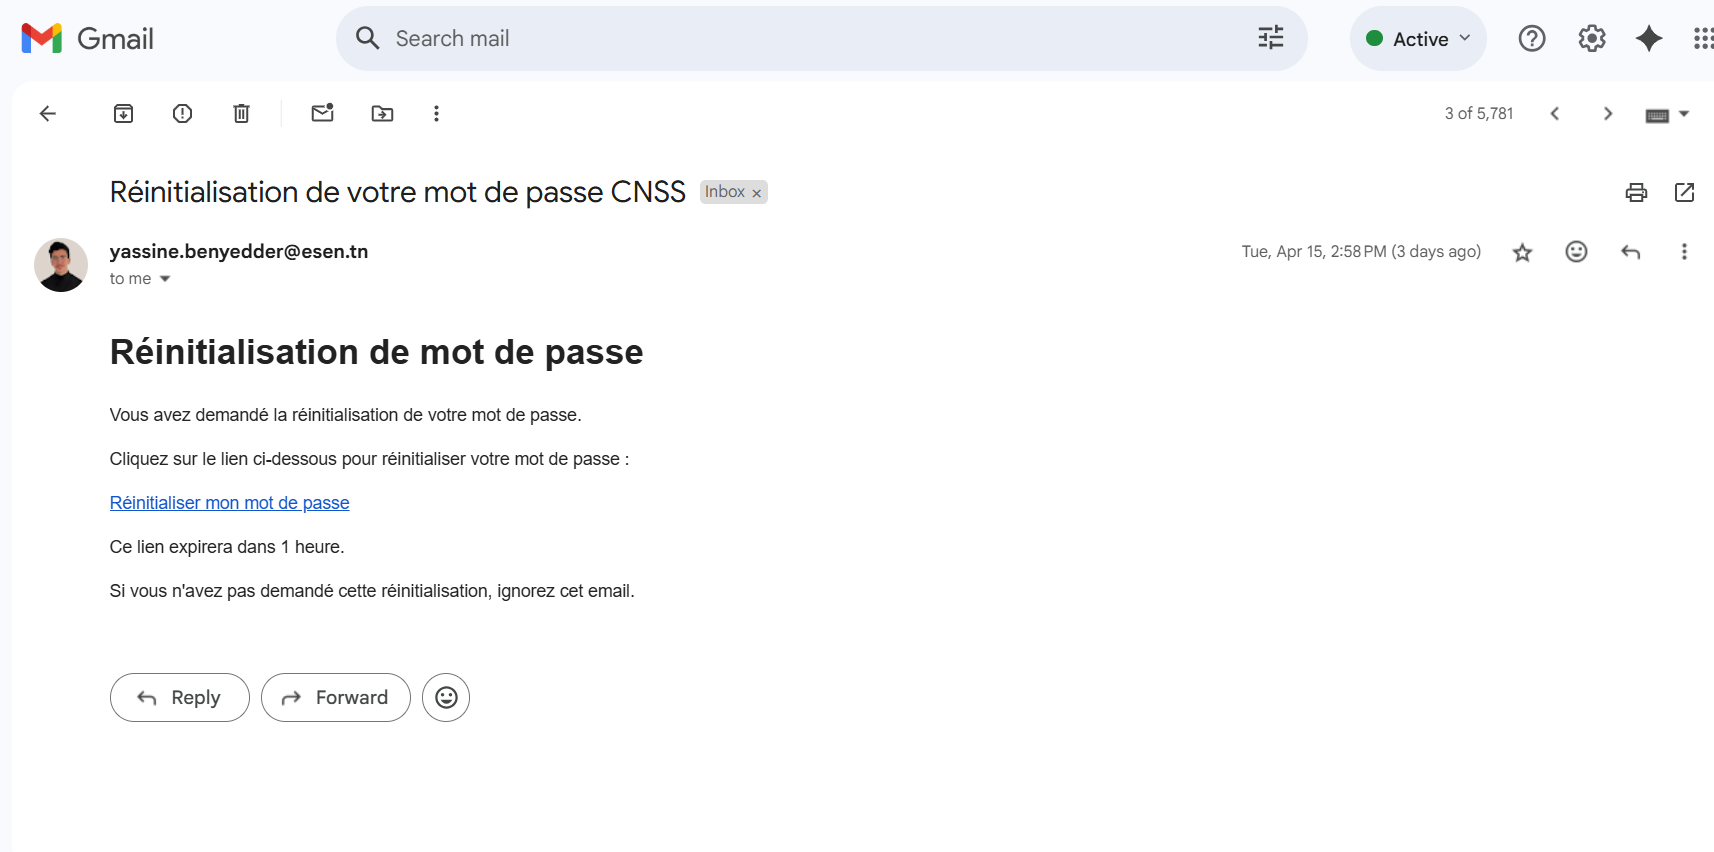
\includegraphics[width=1\textwidth]{figures/ui-reset pass2.png}
    \caption{Interface of resetting password 2.}
\end{figure}
\vspace{1.5cm}
\begin{figure}[h!]
    \centering
    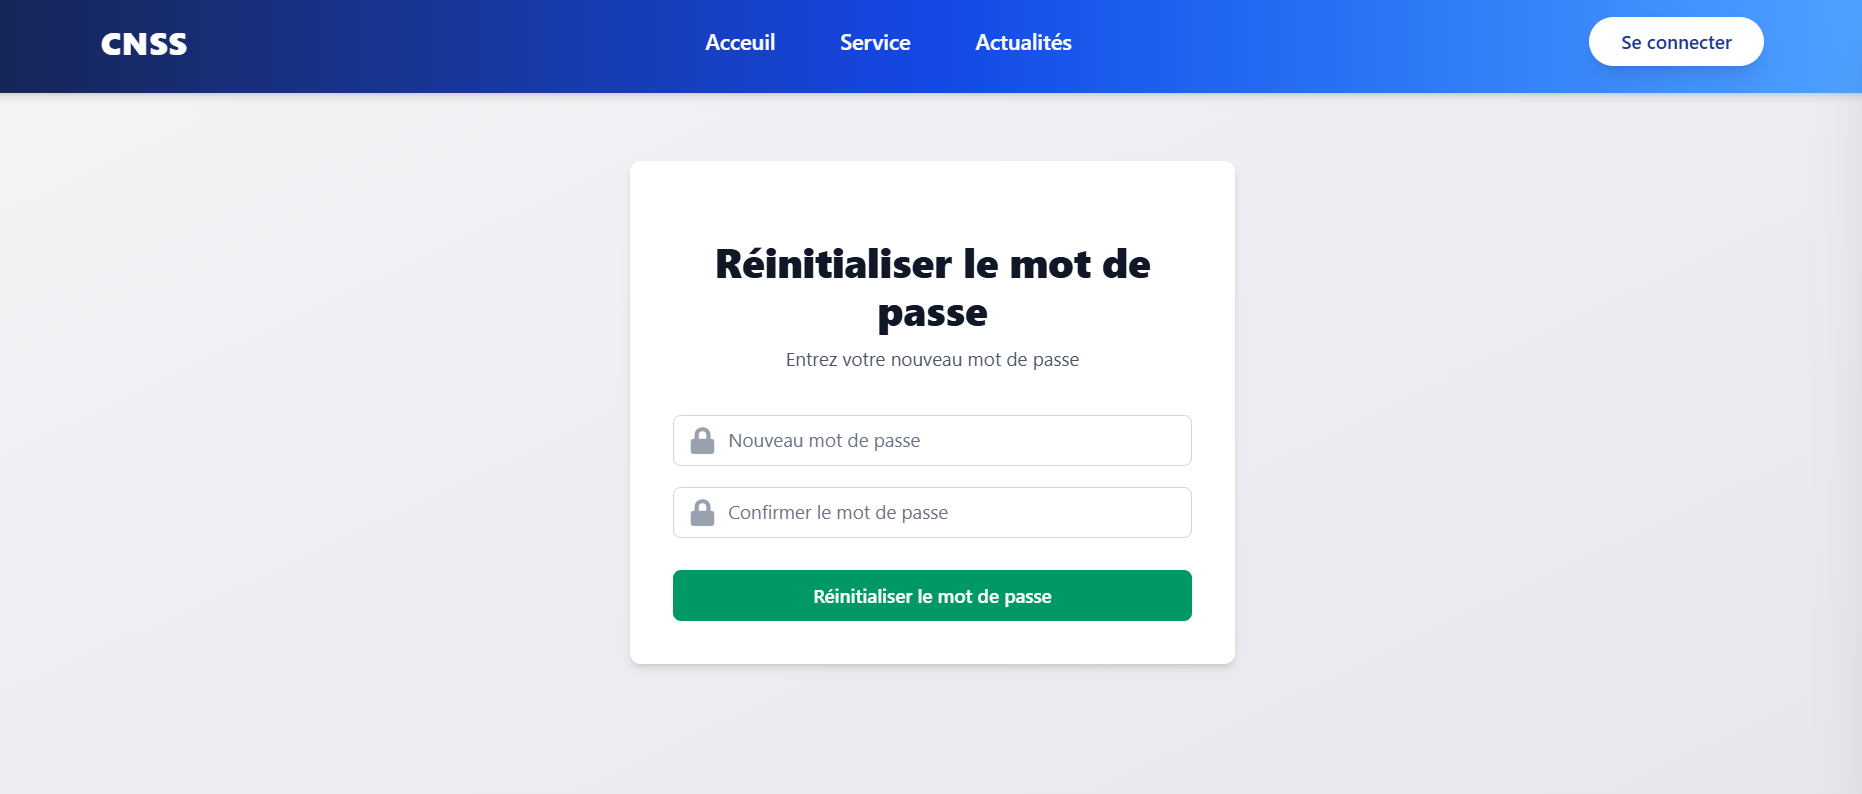
\includegraphics[width=1\textwidth]{figures/ui-reset pass3.png}
    \caption{Interface of resetting password 3.}
\end{figure}
\clearpage
\begin{figure}[h!]
    \centering
    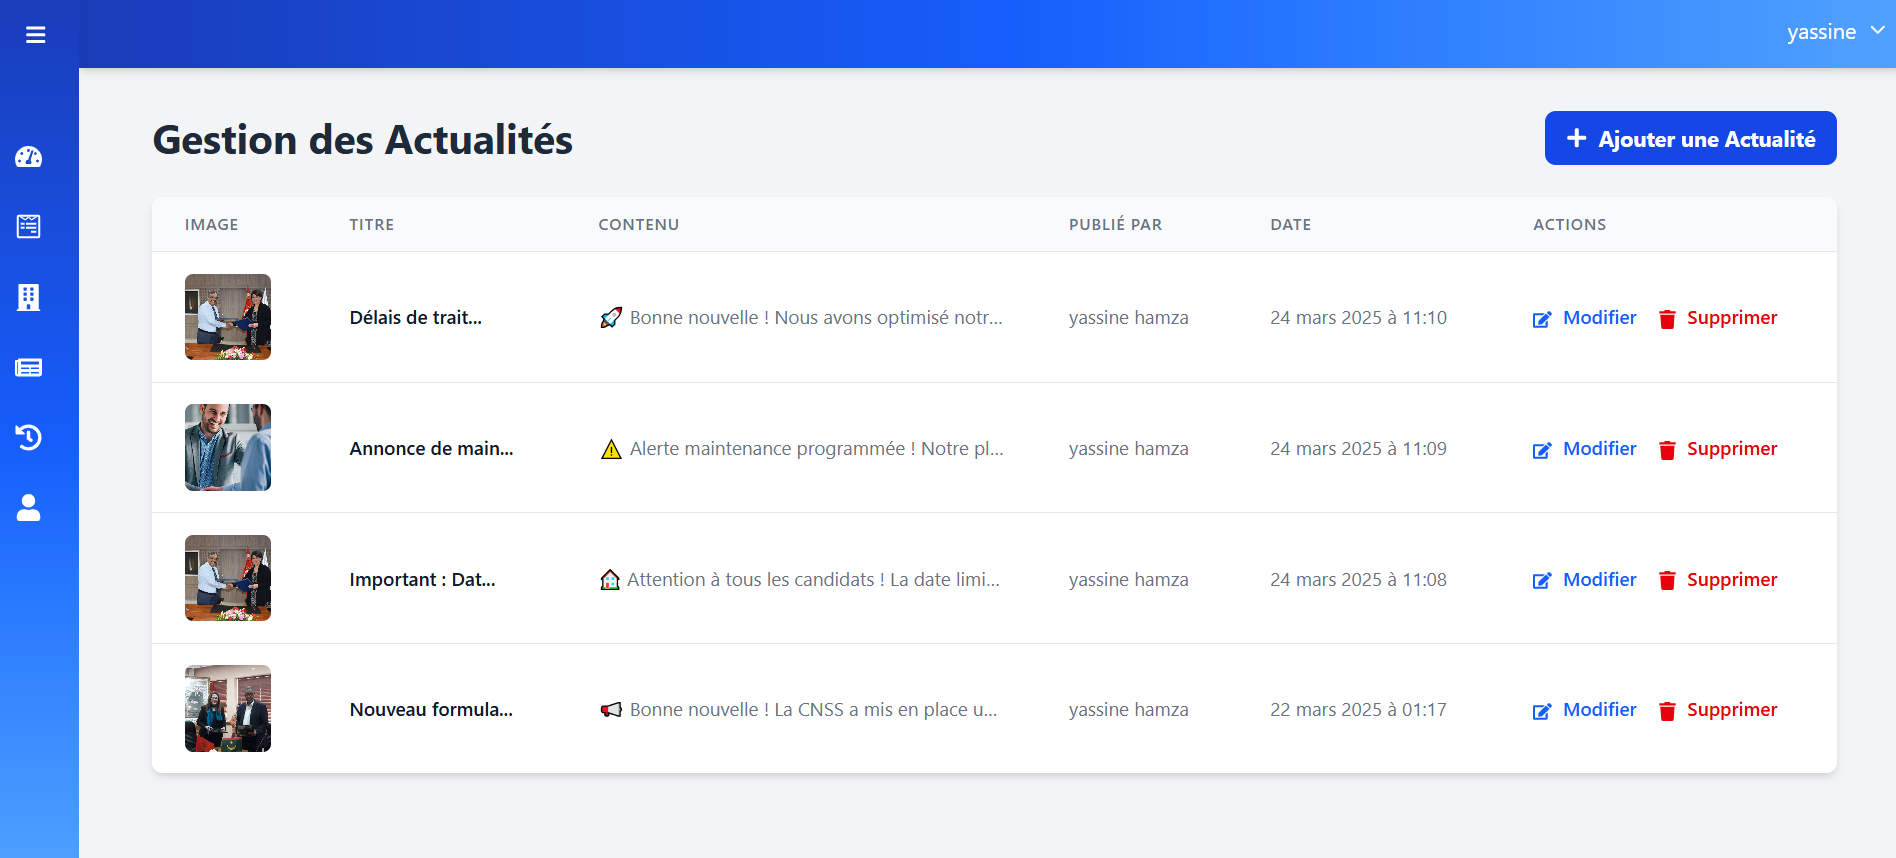
\includegraphics[width=1\textwidth]{figures/ui-manage news.png}
    \caption{Interface of managing the news.}
\end{figure}
\vspace{1.5cm}
\begin{figure}[h!]
    \centering
    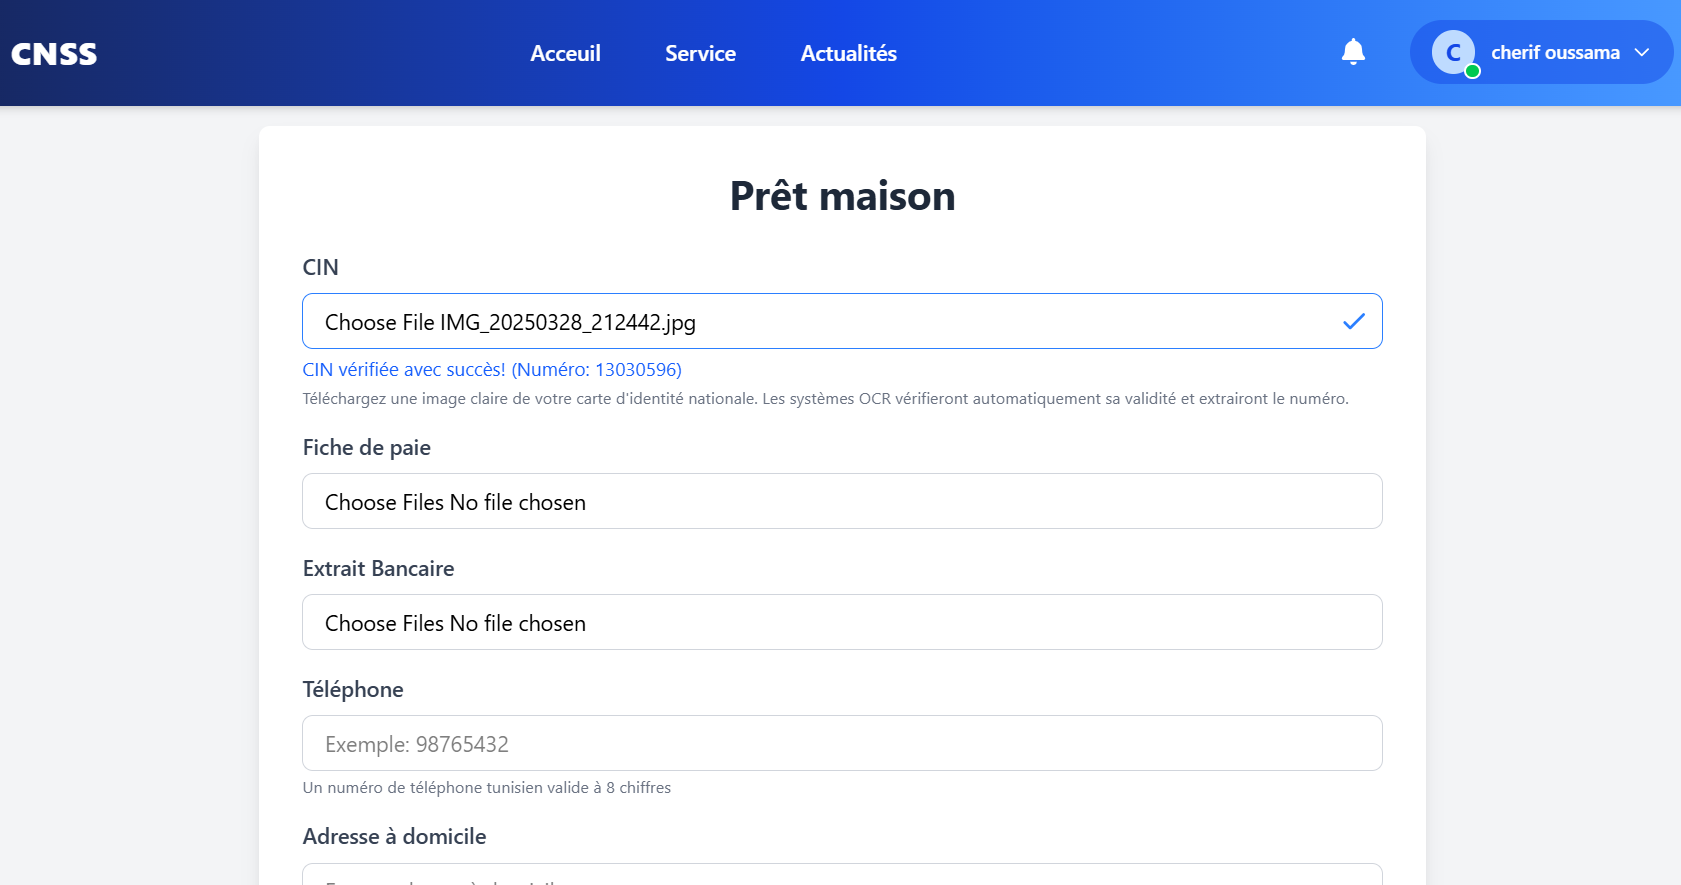
\includegraphics[width=1\textwidth]{figures/ui-recognize ai.png}
    \caption{Interface of the form (recognize documents on file fields).}
\end{figure}
\clearpage
\section{Tests}
During this phase, we will compare the expected results with the actual results.
This will give us the opportunity to ensure the proper functioning of the units (methods) previously implemented.

\subsection{Unit Testing}
We continue to work with the open source Jest unit testing framework to demonstrate in this section some examples of unit tests performed, along with the reasoning behind their implementation.

\subsection{ Unit Test for the Use Case "Create news"}
\subsubsection{Reasoning}
To test the creation of news request, we followed the reasoning below:
\begin{itemize}
    \item Create an object of type News.
    \item Fill in the attributes of the object (e.g., title, content, publication date, author).
    \item Insert the news article into the database.
    \item Test whether the news article was successfully created and stored.
\end{itemize}
\subsubsection{Successful Test Case "Create News"} 
In the case of success, the test performed should return a positive result.
\begin{figure}[h!]
    \centering
    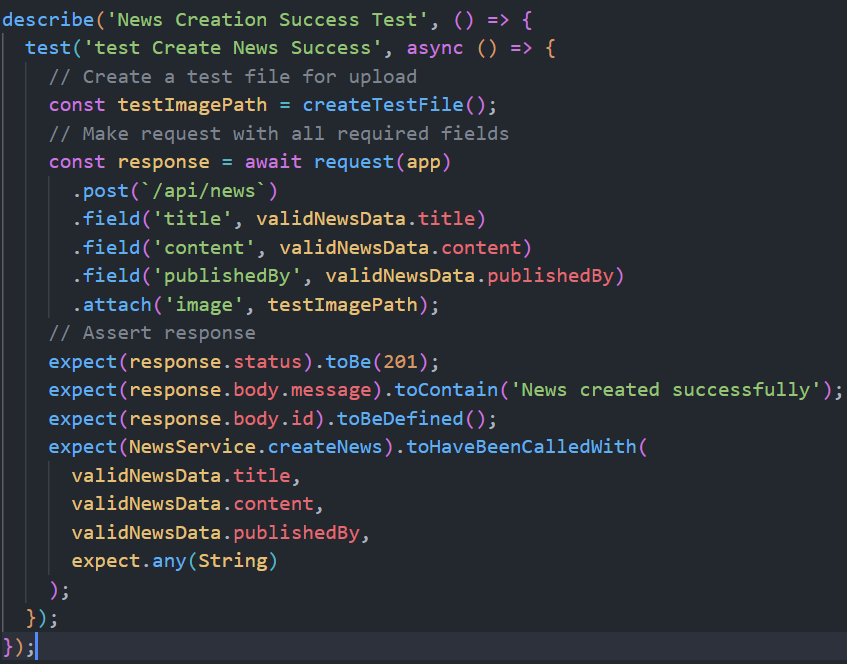
\includegraphics[width=1\textwidth]{figures/create newsS code.png} 
    \caption{Source code of the method create news.}
\end{figure} \
\begin{figure}[h!]
    \centering
    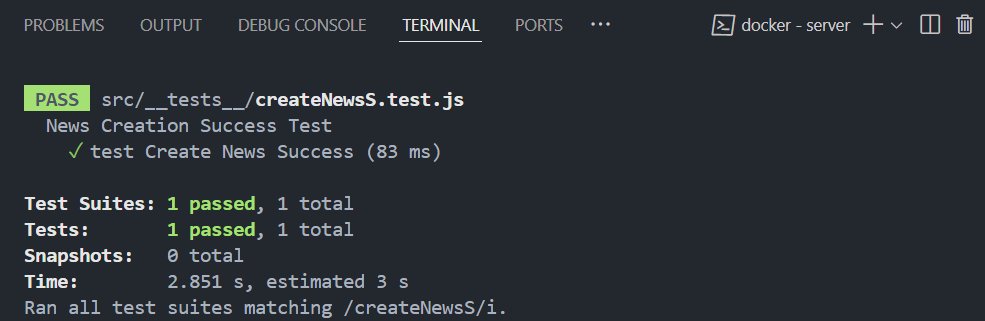
\includegraphics[width=1\textwidth]{figures/result create newsS.png}  
    \caption{Result of the test creating news.}
\end{figure} \
\clearpage
\subsubsection{Failure Test Case "Create News"}
In the case of a fail, the test performed should return a negative result.
\begin{figure}[h!]
    \centering
    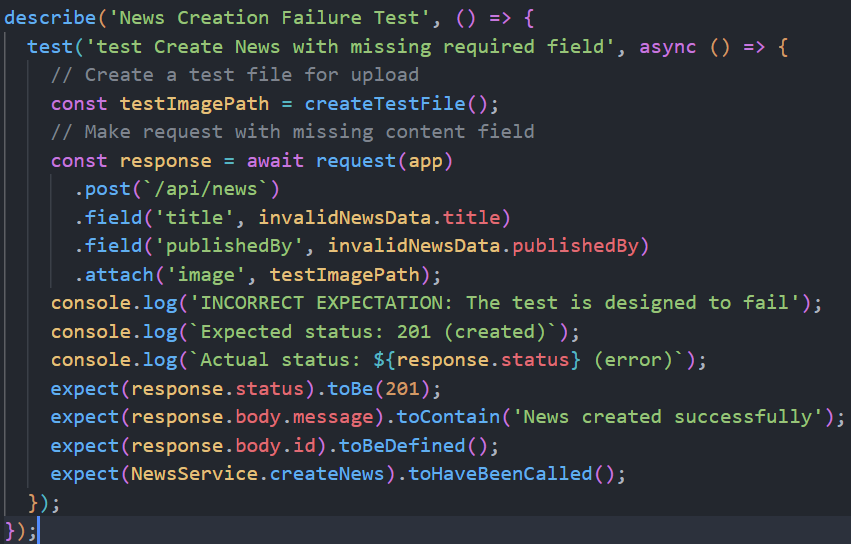
\includegraphics[width=1\textwidth]{figures/create newsF code.png}
    \caption{Source code of the method create news.}
\end{figure} \
\begin{figure}[h!]
    \centering
    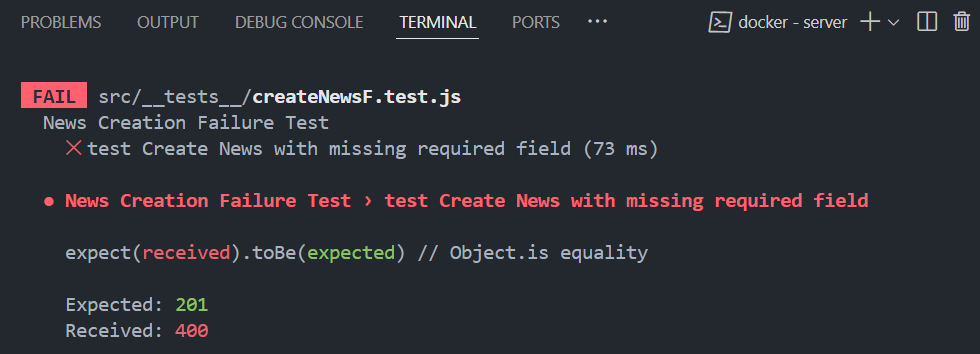
\includegraphics[width=1\textwidth]{figures/result create newsF.png}  
    \caption{Result of the test Creating news.}
\end{figure} \
\clearpage

\subsection{ Unit Test for the Use Case "Validate national identity documents"}
\subsubsection{Reasoning}
To test the validation of the national identity documents request, we followed the reasoning below:
\begin{itemize}
    \item Create an object of type PieceIdentite (IdentityDocument).
    \item Fill in the attributes of the object (e.g., document number, type, expiration date, holder's name).
    \item Apply validation rules (e.g., format checks, expiration status, duplication check).
    \item Test whether the identity document is considered valid or rejected based on the validation logic.
\end{itemize}
\subsubsection{Successful Test Case "Validate national identity documents"} 
In the case of success, the test performed should return a positive result.
\begin{figure}[h!]
    \centering
    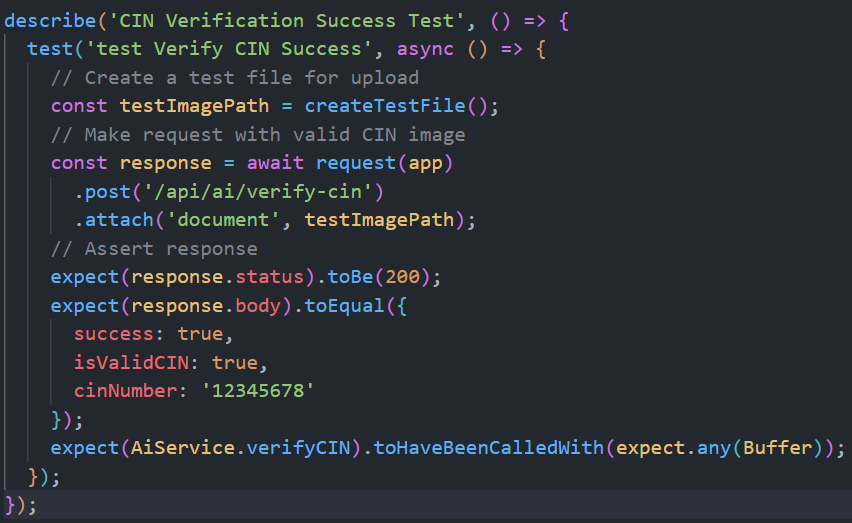
\includegraphics[width=1\textwidth]{figures/validate idS code.png} 
    \caption{Source code of the method Validating national identity documents.}
\end{figure} \
\begin{figure}[h]
    \centering
    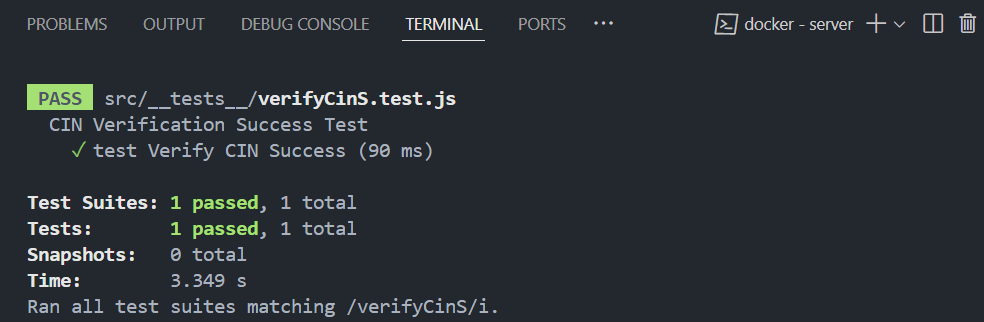
\includegraphics[width=1\textwidth]{figures/result validate national idS.png}  
    \caption{Result of the test Validating national identity documentss.}
\end{figure} \
\
\subsubsection{Failure Test Case "Validate national identity documents"}
In the case of a fail, the test performed should return a negative result.
\begin{figure}[h!]
    \centering
    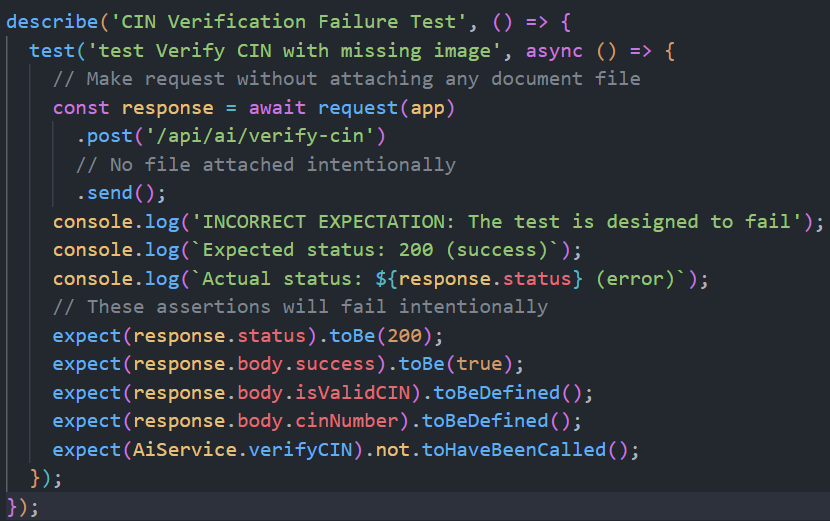
\includegraphics[width=1\textwidth]{figures/validate idF code.png}
    \caption{Source code of the method Validating national identity documents.}
\end{figure} \
\clearpage
\begin{figure}[h!]
    \centering
    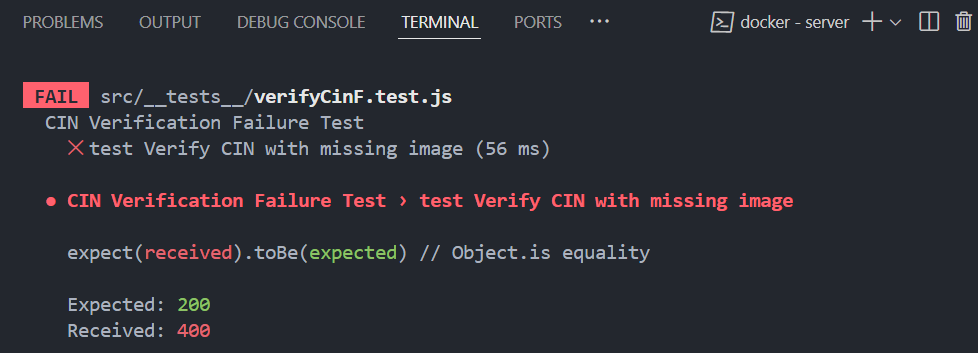
\includegraphics[width=1\textwidth]{figures/result validate national idF.png}  
    \caption{Result of the test Validating national identity documentss}
\end{figure} \

\section{Sprint Review – Burndown Chart Diagram}
The sprint review aims to inspect the results produced during this iteration.
\begin{table}[h!]
\centering
\small
\resizebox{\textwidth}{!}{%
\begin{tabular}{|c|c|c|c|c|c|}
\hline
\textbf{DAY} & \textbf{Hours Planned} & \textbf{Hours Actual} & \textbf{Remaining Planned} & \textbf{Remaining Actual} & \textbf{Done Today} \\
\hline
0  & -  & -  & 160 & 160 & -  \\
1  & 8  & 10 & 152 & 150 & 10 \\
2  & 8  & 10 & 144 & 140 & 10 \\
3  & 8  & 6  & 136 & 134 & 6  \\
4  & 8  & 6  & 128 & 128 & 6  \\
5  & 8  & 10 & 120 & 118 & 10 \\
6  & 8  & 10 & 112 & 108 & 10 \\
7  & 8  & 10 & 104 & 98  & 10 \\
8  & 8  & 10 & 96  & 88  & 10 \\
9  & 8  & 6  & 88  & 82  & 6  \\
10 & 8  & 9  & 80  & 73  & 9  \\
11 & 8  & 7  & 72  & 66  & 7  \\
12 & 8  & 6  & 64  & 60  & 6  \\
13 & 8  & 7  & 56  & 53  & 7  \\
14 & 8  & 8  & 48  & 45  & 8  \\
15 & 8  & 7  & 40  & 38  & 7  \\
16 & 8  & 8  & 32  & 30  & 8  \\
17 & 8  & 8  & 24  & 22  & 8  \\
18 & 8  & 9  & 16  & 13  & 9  \\
19 & 8  & 6  & 8   & 7   & 6  \\
20 & 8  & 9  & 0   & 0   & 9  \\
\hline
\end{tabular}%
}
\caption{Burndown Chart Table for Sprint 3 (20 Days)}
\end{table}
\clearpage
\begin{figure}[h!]
    \centering
    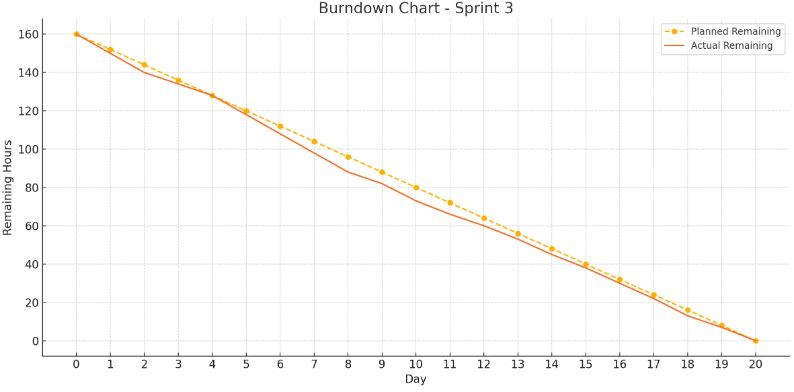
\includegraphics[width=1\textwidth]{figures/burn down chart 3.JPG} 
    \caption{Burn down chart of sprint 3.}
\end{figure} \

\begin{center}
    \doublespacing 
    \centering
    \LARGE\textbf{Conclusion} 
    \vspace{1cm} \\
    \raggedright
\end{center}
\addcontentsline{toc}{section}{Conclusion}
In this chapter, we focused on the development of our Third sprint. As a result, we now have a potentially deliverable increment of our platform.
In the following chapter, we will detail the resources that we used while conducting our project.



